\documentclass[
	% -- opções da classe memoir --
	12pt,				% tamanho da fonte
	openright,			% capítulos começam em pág ímpar (insere página vazia caso preciso)
	oneside,			% para impressão em verso e anverso. Oposto a oneside
	a4paper,			% tamanho do papel.
	% -- opções da classe abntex2 --
	chapter=TITLE,		% títulos de capítulos convertidos em letras maiúsculas
	% section=TITLE,		% títulos de seções convertidos em letras maiúsculas
	%subsection=TITLE,	% títulos de subseções convertidos em letras maiúsculas
	%subsubsection=TITLE,% títulos de subsubseções convertidos em letras maiúsculas
	% -- opções do pacote babel --
	english,			% idioma adicional para hifenização
	%french,				% idioma adicional para hifenização
	%spanish,			% idioma adicional para hifenização
	brazil				% o último idioma é o principal do documento
	]{tcc}


\usepackage{lastpage}			% Usado pela Ficha catalográfica
\usepackage{indentfirst}		% Indenta o primeiro parágrafo de cada seção.
\usepackage{color}				% Controle das cores
\usepackage{graphicx}			% Inclusão de gráficos
\usepackage{microtype} 			% para melhorias de justificação

% ---
% Pacotes de citações
% ---
\usepackage[brazilian,hyperpageref]{backref}	 % Paginas com as citações na bibl
\usepackage[alf]{abntex2cite}	% Citações padrão ABNT

\usepackage{fontspec}
\usepackage[alf]{abntex2cite}
\usepackage{lastpage}
%\usepackage{ifsp-cjo}
\usepackage{graphicx}
\usepackage{float}
\usepackage{indentfirst}
%%%%%%%%%%%%%%%%%%%%%%%%%%%%%%%%%%%%%%%%%
% 				TABELAS					%
%%%%%%%%%%%%%%%%%%%%%%%%%%%%%%%%%%%%%%%%%
\usepackage{tabulary} % Cria tabelas mais facilmente.
\usepackage{booktabs} % Melhora o visual das tabelas.
\usepackage[table]{xcolor} % Pacote de cor pra as tabelas.
\usepackage{caption} % Melhora as legendas de imagens, tabela etc.

%%%%%%%%%%%%%%%%%%%%%%%%%%%%%%%%%%%%%%%%%
% 			CÓDIGO FONTE				%
%%%%%%%%%%%%%%%%%%%%%%%%%%%%%%%%%%%%%%%%%

%Documentação de código fonte.
\usepackage{listings}

%%%%%%%%%%%%%%%%%%%%%%%%%%%%%%%%%%%%%%%%%
% 	Símbolos e Caracteres Matemáticos	%
%%%%%%%%%%%%%%%%%%%%%%%%%%%%%%%%%%%%%%%%%
\usepackage{amsmath}
\usepackage{amssymb}
%\usepackage{amsfonts}
%\usepackage{mathspec} %Habilita o uso das fontes e dos caracteres matematicos.

\usepackage{url} %Facilita o uso de url. Pode-se usar o comando \url{...}.

%%%%%%%%%%%%%%%%%%%%%%%%%%%%%%%%%%%%%%%%%
% 			Configurações				%
%%%%%%%%%%%%%%%%%%%%%%%%%%%%%%%%%%%%%%%%%
\captionsetup{justification=centering,labelfont=bf} %Formata a legenda das figuras.
\graphicspath{{/home/victor/Dropbox/tcc/code/algo_genetico_comum/agc/build-agc-Desktop-Debug/}}

\usepackage{tikz}
\usepackage[hang]{footmisc}
\usepackage{filecontents} %<-- To create the data file on the go
\usepackage{pgfplots}
\pgfplotsset{compat=1.8}
\usepackage{eurosym}      %<-- For EURO symbol 

% --- 
% CONFIGURAÇÕES DE FONTES
% ---
%% Essa linha permite copiar o texto depois que o pdf é gerado.
\usepackage{xltxtra,fontspec,xunicode}

% ---
% Pacotes adicionais, usados apenas no âmbito do Modelo Canônico do abnteX2
% ---
\usepackage{lipsum}				% para geração de dummy text
% ---

\defaultfontfeatures{Ligatures={TeX},Scale={MatchLowercase}}
% \setmonofont{Bitstream Vera Sans Mono}
\setmonofont{Arial}
\setsansfont{Latin Modern Sans} %Source Sans Pro
% \setmainfont{TeX Gyre Pagella}
% \setmainfont{Baskerville}
% \setmainfont{Arial}
% \setmainfont{Comic Sans MS}
\setmainfont{Times New Roman}
%\setmathfont{TeX Gyre Pagella Math}

%%%%% Dados para criação da capa e folha de rosto %%%%
\autor{Victor Hugo Carlquist da Silva}
\titulo{Desenvolvimento de um Algoritmo Genético Híbrido para a solução do problema dos Múltiplos Caixeiros Viajantes (\textit{mTSP})}
\orientador{Prof. Dr. Helton Hugo de Carvalho Júnior}
\coorientador{Prof. Me. André Malvezzi Lopes}
\preambulo{Trabalho de Conclusão de Curso apresentado ao Instituto Federal de Educação, Ciência e Tecnologia - IFSP - \textit{Campus} Campos do Jordão, como parte das exigências para obtenção do título de Tecnólogo em Análise e Desenvolvimento de Sistemas.}
\instituicao{Instituto Federal de Educação, Ciência e Tecnologia de São Paulo}
\local{Campos do Jordão}
\data{7 de janeiro de 2015}

\makeatletter
\hypersetup{
    pdftitle={\@title},
    pdfauthor={\@author},
    pdfsubject={\imprimirpreambulo},
    pdfkeywords={PALAVRAS}{CHAVES}{EM}{PORTUGUES},
    pdfcreator={LaTeX with abnTeX2},
    colorlinks=true,
    linkcolor=black,
    citecolor=black,
    urlcolor=black
}
\makeatother
\definecolor{blues}{rgb}{0.13,0.13,1}
\definecolor{greens}{rgb}{0,0.5,0}
\definecolor{reds}{rgb}{0.9,0,0}

\lstset{language=C++,
basicstyle = \ttfamily\tiny, % Tamanho da fonte do código
numbers = left, % Posição da numeração das linhas
numberstyle = \tiny\color{blue}, % Estilo da numeração de linhas
stepnumber = 0, % Numeração das linhas ocorre a cada quantas linhas?
numbersep = 10pt, % Distância entre a numeração das linhas e o código
backgroundcolor = \color{white}, % Cor de fundo
showspaces = false, % Exibe espaços com um sublinhado
showstringspaces = false, % Sublinha espaços em Strings
showtabs = false, % Exibe tabulação com um sublinhado
frame = , % Envolve o código com uma moldura, pode ser single ou trBL
rulecolor = \color{black}, % Cor da moldura
tabsize = 2, % Configura tabulação em x espaços
captionpos = b, % Posição do título pode ser t (top) ou b (bottom)
breaklines = true, % Configura quebra de linha automática
breakatwhitespace= false, % Configura quebra de linha
%title = \lstname, % Exibe o nome do arquivo incluido
%caption = \lstname, % Também é possível usar caption no lugar de title
keywordstyle = \color{black}, % Estilo das palavras chaves
commentstyle = \color{black}, % Estilo dos Comentários
stringstyle = \color{black}, % Estilo de Strings
escapeinside = {\%*}{*)}, % Permite adicionar comandos LaTeX dentro do seu código
morekeywords     ={*,USE,GO} % Se quiser adicionar mais palavras-chave
}

\usetikzlibrary{chains,fit,shapes}
\usetikzlibrary{fit,arrows,calc,positioning}

%%%%%%%%%%%%%%%%%%%%%%%%%%%%%%%%%%%%%%%%%%%%%%%%%%%%%%%%%
%%%%%%%%%%%%%%%%%%%%%%%%%%%%%%%%%%%%%%%%%%%%%%%%%%%%%%%%%
%%%%%%%%%%%%%%%%%%%%%%%%%%%%%%%%%%%%%%%%%%%%%%%%%%%%%%%%%

\pgfplotsset{every axis legend/.append style={
at={(0,0)},
anchor=north east}} 

\begin{filecontents*}{t1.csv}
Geração Tamanho
0 814906215.827101
232 812626537.581827
470 812356993.636975
709 812076127.172920
960 811835654.870818
1211 811527333.547560
1462 811187618.599136
1712 810912644.778274
1963 810660404.500810
2214 810419055.066827
2465 810140254.759824
2716 809829746.455907
2967 809550105.387874
3217 809248873.778620
3468 809036039.375026
3719 808707054.473107
3970 808439372.735228
4221 808168748.095597
4472 807904631.112837
4714 807651654.208994
4961 807335567.046410
5196 807110864.515245
5441 806820029.828043
5688 806564812.164069
5926 806337460.842033
6170 806093136.580693
6413 805811769.048716
6661 805532298.557325
6911 805264223.724372
7162 804981694.265984
7412 804739123.939362
7663 804480063.584381
7914 804232768.860797
\end{filecontents*}
\begin{filecontents*}{t5.csv}
Geração Tamanho
0 5877651.098502
249 5877651.098502
500 5877651.098502
751 5877651.098502
1002 5877651.098502
1253 5877651.098502
1503 5877651.098502
1754 5877651.098502
2005 5877651.098502
2256 5877651.098502
2507 5877651.098502
2758 5877651.098502
3009 5877651.098502
3260 5877651.098502
3507 5877651.098502
3758 5877651.098502
4009 5877651.098502
4260 5877651.098502
4511 5877651.098502
4762 5877651.098502
5013 5877651.098502
5264 5877651.098502
5515 5877651.098502
5766 5877651.098502
6016 5877651.098502
6262 5877651.098502
6511 5877651.098502
6757 5877651.098502
7005 5877651.098502
7255 5877651.098502
7505 5877651.098502
7751 5877651.098502
7987 5877651.098502
\end{filecontents*}
% exibindo a9-a12  Threads
\begin{filecontents*}{a9.csv}
thread tempo
1 16.577603
2 16.158017
3 16.305763
4 16.223611
5 8 %bug
\end{filecontents*}
\begin{filecontents*}{AG.csv}
Geração Tamanho
0 15242497.826128
7089 12086783.560622
14370 10384073.428560
21512 9417990.635861
28610 8707194.426343
35728 8144479.087712
43052 7718902.290753
50374 7383740.742586
57636 7098353.626970
64791 6864035.999263
71865 6617318.658530
79145 6426306.773559
86372 6259308.682133
93670 6096162.469732
100912 5962287.830430
108170 5821382.833857
114662 5726785.229939
121161 5617619.076104
128095 5543519.826419
135384 5441880.438253
142674 5358664.681169
149666 5279177.210732
157062 5214755.767804
164346 5149341.552654
171165 5089734.976914
178216 5041219.467093
185598 4970110.724457
192970 4913515.381533
200320 4871133.719196
207693 4826935.691453
215085 4771218.216429
222236 4732683.502409
229585 4700641.746658
236932 4640466.009790
244148 4598006.723450
251491 4549817.521288
258903 4505386.605208
266323 4476532.871250
273746 4433032.209641
281170 4397624.143006
288597 4367262.972514
296025 4331075.908366
303451 4306262.771030
310873 4279134.302584
318298 4260547.821134
325721 4225650.837000
333135 4202126.549665
340557 4180463.490231
347976 4155983.981219
355403 4135550.606787
362831 4113445.774628
370187 4092617.299120
377442 4070606.608332
384845 4053206.456751
392249 4034129.978636
399652 4013540.579058
407055 3992821.976135
414459 3973978.852466
421872 3943614.621519
429284 3922211.657545
436693 3896188.833619
444104 3880637.848359
451517 3864094.551441
458932 3845152.170465
466342 3822093.264160
473757 3804035.476905
481173 3790637.004471
488586 3775748.722122
496002 3763836.858299
503415 3748598.246987
510822 3729877.658710
518241 3718709.693614
525649 3701476.710969
533052 3688893.063018
540268 3674296.161014
547606 3662985.411782
554856 3649774.503650
562157 3636573.585716
569576 3626568.660661
576996 3615343.891947
584416 3603513.518715
591835 3592170.618934
599256 3582644.893317
606678 3572354.917685
614096 3562638.067710
621522 3550578.928081
628941 3542157.233017
636367 3533369.295472
643778 3519459.151214
651119 3503294.602376
658488 3495077.335376
665903 3486449.273503
673304 3479428.151169
680712 3475104.934469
688119 3465367.549139
695528 3460066.994296
702932 3450128.100713
710340 3442309.911074
717758 3430063.908903
725180 3422206.420913
732591 3414633.393406
740013 3405820.632173
747434 3396677.861954
754696 3390912.167424
761951 3384129.335782
769256 3376868.292251
776446 3372504.436201
783712 3366688.853847
790857 3357824.234469
798188 3349127.203553
805442 3339848.135190
812810 3333315.746574
820224 3326701.056443
827628 3322508.386587
834857 3315809.683002
842245 3308420.124416
849595 3300073.621132
856953 3290997.233128
864312 3284013.762362
871676 3277812.084410
878724 3272123.080338
886049 3267579.822842
893323 3262183.989271
900736 3256552.650708
908146 3248206.178175
915565 3240894.518741
922983 3235645.942266
930405 3230793.906960
937825 3224203.917248
945244 3216763.984978
952663 3208786.330367
960089 3202863.635318
967483 3199552.122740
974909 3191804.572028
982333 3188100.067624
989758 3181689.269832
997053 3178467.544356
1004379 3174061.000114
1011796 3166986.219316
1019220 3161081.483071
1026639 3157864.235652
1034064 3153356.548740
1041485 3144529.839721
1048911 3139713.891838
1056340 3132803.166837
1063759 3124102.286683
1071179 3114872.597040
1078589 3107066.106249
1086006 3103181.904519
1093425 3100035.405419
1100837 3097198.523057
1108260 3092431.731203
1115672 3089316.315412
1123042 3082392.486960
1130309 3078570.601579
1137606 3074336.649368
1145017 3066505.624297
1152439 3059993.175313
1159855 3056494.720179
1167265 3051193.422549
1174672 3046507.370279
1182099 3042909.679262
1189517 3034945.908534
1196943 3031153.043485
1204364 3026774.120167
1211789 3020605.015987
1219214 3017098.330903
1226643 3012631.885033
1234071 3007525.350130
1241494 3003612.880806
1248911 3000629.369712
1256327 2997055.157765
1263548 2994006.906066
1270953 2990151.100694
1278376 2984871.441357
1285796 2982259.298153
1293216 2979549.543800
1300641 2974935.482909
1308065 2969686.431335
1315488 2965755.698061
1322915 2960287.201020
1330343 2957852.288766
1337768 2952416.913870
1345189 2949297.461135
1352601 2945696.248468
1359983 2940702.615546
1367273 2935756.316241
1372876 2934719.813962
1378420 2933576.748963
1383979 2932070.454533
1389533 2927612.384771
1395089 2925349.886052
1400645 2923869.070394
1406210 2920605.007722
1411775 2917385.883593
1417341 2913766.240636
1422844 2911873.110615
1428356 2910080.088000
1433931 2907905.866916
1439502 2905359.975617
1445074 2902684.734548
1450649 2899460.997561
1456224 2897562.521726
1461797 2893513.032799
1467374 2890602.244356
1472951 2890310.164129
1478527 2889046.100621
1484085 2885363.415518
1489651 2882054.535606
1495213 2879253.860224
1500786 2877004.422595
1506362 2876344.639069
1511932 2874702.862821
1517506 2871570.124621
1523074 2870686.579756
1528650 2869372.296478
1534221 2866568.690543
1539796 2865071.333646
1545374 2864067.103535
1550950 2862595.846276
1556512 2858551.718614
1562078 2856314.398024
1567641 2853585.557787
1573210 2851627.808261
1578784 2847512.394077
1584362 2846558.992584
1589937 2844993.305208
1595512 2843377.094363
1601088 2842339.504733
1606660 2841646.160435
1612218 2839404.105661
1617775 2837400.489120
1623322 2834361.175519
1628879 2832131.556740
1634444 2831000.050821
1640012 2828389.802314
1645584 2827539.556874
1651160 2826595.027458
1656734 2824702.546804
1662308 2823743.751765
1667884 2823158.900380
1673458 2822538.220244
1679034 2821439.173148
1684605 2819219.561888
1690181 2818172.492814
1695754 2816621.714601
1701328 2813257.429978
1706903 2812120.328058
1712478 2810654.452475
1718054 2807232.645778
1723618 2805657.104731
1729186 2802472.526866
1734752 2801853.181078
1740318 2800385.189439
1745892 2798753.561486
1751467 2796481.924034
1757042 2794566.082153
1762612 2791492.261940
1768188 2789847.653621
1773762 2788382.641440
1779337 2786280.497279
1784913 2784875.982125
1790490 2783391.978020
1796063 2780098.432660
1801636 2771693.414720
1807214 2769713.519902
1812788 2768369.952081
1818364 2765781.621103
1823941 2762252.360737
1829516 2761039.964750
1835088 2759368.581562
1840653 2758732.124738
1846211 2757727.275897
1851780 2756952.539676
1857356 2755717.204283
1862931 2754847.951278
1868501 2753721.245033
1874076 2752073.159805
1879655 2749537.317636
1885231 2748568.932844
1890805 2748017.362312
1896381 2746380.644743
1901959 2745275.378740
1907538 2743949.142991
1913115 2741944.782404
1918693 2741053.334762
1924271 2739328.990469
1929832 2738141.237433
1935399 2735702.513523
1940962 2734239.120855
1946532 2732336.572327
1952095 2731676.103372
1957661 2731122.992426
1963230 2728925.111361
1968808 2728188.207983
1974389 2726904.591393
1979964 2725488.414421
1985538 2724762.373884
1991108 2724006.330225
1996676 2723300.271488
2002246 2719846.399047
2007816 2719353.692662
2013388 2716585.533526
2018959 2714704.996036
2024533 2711982.143167
2030112 2711130.847277
2035688 2710482.839383
2041251 2709615.855976
2046818 2707693.229623
2052391 2705582.394310
2057966 2703404.679400
2063539 2702627.494934
2069116 2702161.796386
2074657 2701187.443403
2080223 2699659.143586
2085782 2697945.899285
2091070 2696860.122025
2096591 2695496.518423
2102165 2694583.832195
2107738 2691093.668291
2113308 2689762.043534
2118881 2687874.094356
2124454 2686526.276671
2130029 2685785.928851
2135291 2683491.955665
2140713 2681473.750059
2146289 2679284.942248
2151863 2678860.287279
2157436 2677628.303760
2163008 2676786.267758
2168432 2675843.966894
2173852 2674916.963824
2179273 2673953.952307
2184848 2672716.382846
2190121 2671451.789325
2195698 2671151.397687
2201273 2670486.244960
2206840 2669246.345556
2212414 2667650.231303
2217986 2665531.419488
2223407 2663182.229395
2228828 2661756.227800
2234254 2660222.550015
2239830 2658310.711590
2245096 2657217.942530
2250668 2655726.871400
2255942 2655074.070592
2261363 2654534.765865
2266787 2653922.086818
2272208 2652980.283527
2277479 2652050.911184
2282902 2650822.544035
2288170 2650318.891614
2293747 2648133.790066
2299013 2647913.608783
2304434 2646729.926564
2309858 2646286.254093
2315285 2645701.371550
2320712 2644405.286227
2326135 2644180.546253
2331553 2643452.034267
2337132 2642494.807128
2342555 2640340.272519
2347977 2640333.779647
2353401 2638624.625032
2358824 2637545.319206
2364250 2637427.002707
2369820 2635214.735036
2375388 2633807.335639
2380950 2632337.466349
2386517 2631244.691735
2391946 2630253.486231
2397205 2626166.900871
2402562 2624658.374533
2408144 2622291.869504
2413725 2622027.942880
2419303 2621351.395809
2424876 2620589.097532
2430148 2619914.474625
2435575 2619434.577562
2440998 2619162.131677
2446571 2618718.879671
2452145 2617040.785942
2457720 2616531.076633
2463144 2614837.917918
2468722 2613704.013433
2474146 2613140.634003
2479728 2611981.510751
2485154 2611121.868432
2490729 2609076.441904
2496155 2607853.171454
2501582 2607015.924784
2507009 2605583.258880
2512580 2603773.669984
2518148 2603192.665378
2523705 2602114.311816
2529272 2601043.246403
2534836 2599367.164307
2540406 2598090.044359
2545975 2596717.711015
2551547 2595965.132868
2557123 2594868.752934
2562691 2594260.016351
2568261 2594130.056596
2573820 2593478.781937
2579384 2592661.384472
2584945 2591850.865902
2590515 2591465.319393
2596085 2590453.911389
2601657 2589580.767176
2607222 2588257.173278
2612787 2586967.081716
2618348 2585492.387077
2623906 2584455.451639
2629476 2583161.080660
2635047 2579575.043977
2640615 2578466.409319
2646177 2578006.825922
2651751 2577055.480333
2657325 2577050.811896
2662741 2576532.046311
2668163 2574859.008564
2673588 2574325.547648
2679012 2572963.003035
2684398 2571278.911109
2689976 2570837.495422
2695403 2569756.576843
2700824 2568557.041977
2706247 2567678.779297
2711824 2566216.027251
2717242 2565625.598427
2722817 2564722.215731
2728390 2563971.503579
2733964 2562976.288286
2739220 2562387.510716
2744691 2561902.527381
2750220 2561612.548292
2755789 2560248.546703
2761368 2560150.791092
2766950 2559637.212694
2772516 2558756.171948
2778090 2557703.657127
2783661 2557135.506236
2789233 2556632.656347
2794803 2555945.810284
2800370 2555697.285916
2805944 2555204.904283
2811511 2554292.799197
2817088 2553923.455381
2822659 2553453.507735
2828230 2552054.128992
2833799 2551474.390492
2839371 2550665.404644
2844942 2550066.745868
2850521 2549781.030371
2856098 2548716.564909
2861674 2547490.033866
2867252 2547306.178998
2872835 2546327.776308
2878412 2546020.395870
2883981 2545591.320232
2889552 2544889.673848
2895124 2544273.389451
2900697 2543992.064667
2906272 2543766.291473
2911842 2542762.527315
2917416 2542201.394177
2922987 2541613.511031
2928564 2540452.723071
2934134 2540211.891360
2939707 2539351.734468
2945280 2538100.323717
2950852 2537588.286966
2956431 2536986.384900
2961882 2536778.591253
2967365 2536593.230523
2972939 2535999.734467
2978502 2535347.865497
2984074 2534743.214490
2989638 2534424.536493
2995211 2533916.078640
3000789 2533231.624862
3006371 2532426.143661
3011949 2531426.127610
3017520 2530938.968703
3023076 2530340.247047
3028645 2530059.779820
3034217 2529670.959432
3039797 2528264.744374
3045380 2527818.647007
3050955 2527497.255952
3056530 2527070.012863
3062098 2526774.051566
3067663 2526527.067486
3073232 2526029.002138
3078799 2525595.445606
3084281 2524908.185950
3089853 2523680.452315
3095435 2523380.255136
3101018 2522631.439930
3106593 2521684.615818
3112168 2519850.761964
3117733 2519165.003401
3123300 2519003.818911
3128881 2518421.639883
3134460 2516955.098524
3140043 2516501.142694
3145615 2516070.514650
3151194 2515936.045461
3156772 2514795.060833
3162343 2513893.320796
3167916 2513358.888941
3173484 2513064.381805
3179059 2512446.353182
3184511 2512122.707735
3190083 2511171.509585
3195648 2510853.446480
3201220 2509109.388828
3206799 2508235.349258
3212378 2507953.012548
3217959 2507531.066837
3223538 2506657.279672
3229120 2506526.392486
3234699 2506123.313064
3240260 2505867.903858
3245829 2505654.045252
3251401 2504507.160812
3256972 2504028.144925
3262550 2502532.080311
3268128 2502092.531095
3273711 2501451.269537
3279291 2500690.212998
3284865 2499824.106016
3290441 2499454.628059
3296004 2498384.765682
3301574 2497959.672168
3307145 2497871.126628
3312710 2496389.947883
3318289 2496181.359305
3323865 2495609.128111
3329443 2495469.211621
3335024 2494947.133141
3340604 2494343.067579
3346180 2493121.616963
3351750 2491916.277328
3357318 2491265.512626
3362894 2489997.862608
3368466 2488347.527933
3374044 2487346.557254
3379623 2486979.504757
3385203 2485209.337746
3390781 2484887.910397
3396362 2484369.593135
3401944 2483829.342007
3407467 2482940.510939
3413029 2481960.350839
3418567 2481549.381440
3424130 2480626.606550
3429706 2480197.717699
3435282 2479913.418818
3440858 2479619.802218
3446428 2479393.127605
3452004 2479362.926084
3457581 2478254.050826
3463147 2476544.483432
3468725 2476511.442961
3474296 2476474.891967
3479737 2476330.333127
3485106 2476094.240681
3490682 2475624.033433
3496264 2475374.851271
3501721 2475183.587128
3507278 2474804.567842
3512858 2474550.403834
3518434 2474419.584429
3523866 2473938.196068
3529442 2472642.209935
3535016 2472444.181364
3540592 2471343.576215
3546171 2470945.118688
3551749 2470057.904817
3557325 2469532.499913
3562906 2469114.404800
3568486 2468587.879845
3574054 2468321.608977
3579623 2468103.223513
3585202 2467336.004367
3590770 2466984.487348
3596340 2466775.318519
3601916 2465635.018834
3607496 2465356.236368
3613072 2461174.669071
3618644 2460678.928445
3624222 2459701.480066
3629469 2459395.127967
3635049 2458615.011444
3640624 2457781.005326
3646196 2457516.090905
3651771 2457112.422541
3657341 2456327.425991
3662918 2456285.606620
3668488 2455533.646270
3674059 2455164.272577
3679637 2454094.325432
3685207 2453554.764129
3690778 2453243.437548
3696349 2453048.111248
3701921 2452993.745077
3707503 2452190.698115
3713078 2452034.279687
3718659 2451814.069403
3724234 2451440.369237
3729809 2450707.824465
3735386 2450247.201045
3740956 2449753.765573
3746531 2449641.409586
3752102 2449331.557382
3757660 2448409.421252
3763232 2447611.693149
3768804 2447493.199953
3774380 2446871.988425
3779956 2446111.660939
3785539 2446015.745406
3791123 2445694.092646
3796691 2445222.394212
3802263 2444513.549388
3807836 2443218.722460
3813315 2442753.475251
3818656 2442742.993841
3824229 2442511.345239
3829796 2442039.105410
3835362 2441389.429932
3840927 2441141.028994
3846493 2438413.489914
3851947 2436938.566960
3857521 2436451.653735
3863096 2436039.358741
3868671 2435496.148138
3874251 2434984.007540
3879832 2433485.068156
3885412 2432869.665085
3890990 2431645.157994
3896562 2431494.715766
3902132 2431260.993683
3907696 2430165.386439
3913267 2429722.228449
3918837 2429088.394414
3924326 2428141.222463
3929906 2427892.210182
3935483 2427227.048277
3941061 2427226.904735
3946640 2426801.106978
3952215 2426749.048663
3957797 2426242.907252
3963364 2425425.449184
3968936 2424473.995689
3974509 2423649.234229
3980084 2421601.106443
3985664 2421234.715212
3991245 2421234.715212
3996822 2421079.094639
4002389 2420418.131654
4007958 2419784.823790
4013533 2419784.823790
4019101 2418688.094276
4024682 2418462.190999
4030261 2418256.037683
4035828 2417676.012762
4041402 2416730.135155
4046974 2416046.920029
4052550 2415594.997972
4058125 2415137.688289
4063698 2414887.981664
4069277 2414701.845902
4074857 2414424.361901
4080427 2414233.451812
4085996 2413137.830205
4091563 2413095.215063
4097135 2412480.244443
4102698 2412446.045673
4108264 2412050.304047
4113827 2412045.960983
4119396 2411627.000652
4124964 2410441.443956
4130533 2409981.629237
4136107 2408720.393221
4141680 2408407.406888
4147243 2407813.960282
4152814 2407477.353411
4158377 2406438.071000
4163949 2405742.963215
4169521 2405488.925651
4175085 2405169.300228
4180662 2404936.695439
4186235 2403976.492609
4191803 2403847.508729
4197368 2403558.343939
4202936 2403558.343939
4208507 2403477.742675
4214074 2403112.863411
4219642 2402686.062486
4225206 2402351.191496
4230773 2402104.355746
4236354 2401955.653620
4241641 2401861.752759
4247167 2400983.738433
4252663 2400666.696786
4258236 2399901.276150
4263816 2399711.938473
4269391 2399440.530027
4274970 2399029.173895
4280542 2398357.337299
4286119 2397688.557990
4291698 2396803.540463
4296940 2396651.614472
4302508 2396629.585884
4308072 2396176.587294
4313629 2395899.352977
4319195 2395671.934338
4324749 2395147.577783
4330322 2395127.950637
4335895 2394211.162002
4341469 2394029.855969
4347039 2393651.067149
4352608 2393597.673488
4358181 2393479.550875
4363754 2393315.116401
4369320 2392879.985501
4374890 2392406.051397
4380462 2392027.474570
4386034 2391378.464718
4391606 2391358.433391
4397176 2390871.034207
4402756 2390683.192628
4408338 2390356.458593
4413919 2390098.641795
4419499 2389150.264304
4425074 2388933.777515
4430659 2388701.174467
4436245 2387852.733520
4441824 2387852.733520
4447386 2387266.740720
4452966 2387090.517637
4458542 2386174.239701
4464125 2386037.718541
4469706 2384669.869205
4475289 2384361.974031
4480866 2384228.512000
4486449 2384033.246575
4492033 2383554.583801
4497616 2383216.926322
4503189 2383029.586209
4508753 2382893.703359
4514330 2382091.554831
4519905 2381894.710695
4525488 2381200.705006
4531075 2380734.029337
4536644 2380472.262722
4542220 2380392.365271
4547787 2379966.009699
4553362 2379795.922707
4558946 2379714.329343
4564530 2379557.508726
4570114 2379165.967703
4575681 2378481.808735
4581257 2378152.871516
4586834 2376505.125589
4592406 2376338.629432
4597991 2376086.520338
4603574 2375926.482436
4609159 2375893.057841
4614746 2375417.050714
4620326 2375287.299836
4625909 2375284.349729
4631480 2375191.293138
4637058 2375059.546931
4642625 2374724.268961
4648192 2374495.608095
4653778 2373986.065993
4659363 2373440.953901
4664947 2373401.662617
4670533 2372455.672114
4676119 2371745.999648
4681701 2371724.088255
4687269 2371478.331343
4692840 2371378.956439
4698418 2371180.762599
4703987 2370707.005872
4709475 2370036.473468
4714932 2369934.651606
4720391 2369871.941357
4725877 2369687.395669
4730005 2369546.580475
4735587 2368766.227841
4741047 2368499.610933
4746508 2368199.689979
4752083 2367303.468848
4757656 2366957.454563
4763231 2366418.192842
4768809 2366416.894305
4774391 2366047.690492
4779966 2365426.908793
4785545 2365426.908793
4791128 2365218.353058
4796712 2364932.878919
4802297 2364866.419043
4807883 2364774.799533
4813457 2364501.254466
4819034 2364057.668131
4824611 2363313.173837
4830192 2363236.619520
4835773 2362469.734746
4841305 2362272.144230
4846887 2361882.369892
4852461 2361403.142034
4858044 2360472.281325
4863619 2360349.006499
4869196 2359659.606614
4874780 2358575.582202
4880363 2358319.604929
4885948 2358178.359132
4891520 2357997.030805
4897089 2357252.859224
4902663 2357197.156688
4908242 2357038.186557
4913829 2356936.357523
4919408 2356873.797215
4924980 2356371.686222
4930554 2355842.681058
4936007 2355841.151699
4941585 2355525.440761
4947167 2355020.211728
4952748 2354615.362084
4958330 2354485.643637
4963705 2353964.303214
4969245 2353796.723953
4974826 2353353.164028
4980380 2353220.577035
4985950 2353183.219032
4991521 2352700.981304
4997093 2352416.334309
5002679 2352195.710514
5008254 2351583.362641
5013840 2351453.844136
5019409 2350986.170857
5024980 2350944.096609
5030545 2350676.797235
5036110 2350638.468724
5041679 2350085.566399
5047230 2349361.981129
5052801 2349113.847242
5058382 2349060.992104
5063964 2349052.178904
5069545 2348894.898427
5075115 2348427.655655
5080684 2348208.451177
5086219 2348030.068619
5091780 2347995.219870
5097335 2347462.463525
5102900 2346952.165573
5108469 2346228.976585
5114043 2346011.540270
5119625 2345522.936915
5125205 2345380.245920
5130780 2345073.958385
5136354 2344615.378669
5141925 2344364.815827
5147494 2343781.301576
5152924 2343714.431696
5158505 2343519.701872
5164088 2343225.817920
5169658 2342846.370900
5175233 2342548.676841
5180809 2341732.811446
5186180 2341675.324914
5191759 2341397.645800
5197331 2341320.699029
5202906 2340810.650584
5208493 2340676.826188
5214079 2340480.605820
5219665 2340220.165703
5225249 2339253.295589
5230833 2338920.848547
5236421 2338920.848547
5242010 2338015.748306
5247593 2337712.234473
5253181 2337575.633986
5258752 2337417.100661
5264331 2337195.184589
5269909 2336828.958120
5275490 2336558.717360
5281071 2335840.553274
5286647 2335752.280565
5292221 2334922.517126
5297795 2334715.625908
5303371 2334714.098576
5308945 2334217.686929
5314522 2333566.876433
5320106 2333505.773144
5325680 2332627.249314
5331262 2332010.348970
5336833 2331727.795921
5342404 2331131.632397
5347985 2329961.979090
5353556 2329840.958677
5359134 2329584.049578
5364709 2328828.781680
5370280 2328559.544192
5375864 2328287.649480
5381448 2328285.967380
5387033 2328163.844590
5392602 2327849.720624
5398181 2327793.305787
5403740 2327633.949216
5409079 2327484.215989
5414653 2326909.585012
5420231 2326833.072566
5425803 2326520.291472
5431374 2325894.949210
5436942 2325142.339671
5442519 2324908.211431
5448098 2324897.710363
5453680 2324589.965432
5459262 2324430.114330
5464838 2323887.943911
5470414 2323523.587414
5475984 2323372.581035
5481558 2323068.071232
5487142 2322971.471971
5492722 2322902.926777
5498289 2322719.627669
5503858 2322358.469157
5509442 2322229.940134
5515023 2322226.771070
5520609 2321847.585838
5526182 2321751.495784
5531750 2319553.096184
5537325 2319430.054846
5542895 2318640.908559
5548472 2318498.489704
5554038 2318067.702098
5559608 2317876.509090
5565167 2317793.775973
5570740 2317485.685101
5576305 2317475.916806
5581877 2317368.449809
5587447 2317113.845764
5593012 2316901.229094
5598574 2316708.082485
5604138 2316525.336902
5609701 2316385.903376
5615267 2316141.041538
5620830 2316077.976021
5626381 2316028.204977
5631924 2315615.939051
5637473 2315352.614322
5643062 2315137.266578
5648633 2314624.112784
5654215 2314564.192728
5659797 2314260.874773
5665380 2313761.845564
5670971 2313628.191802
5676553 2313350.465390
5682140 2313294.027915
5687713 2313292.728589
5693293 2312981.668015
5698870 2312981.668015
5704452 2312911.616366
5710035 2312736.599094
5715605 2312618.162163
5721169 2312143.292722
5726736 2312143.292722
5732298 2312080.413065
5737835 2312080.413065
5743402 2311669.258352
5748972 2311428.659363
5754532 2311342.015319
5759977 2311068.303795
5765553 2310680.484430
5771124 2310614.979288
5776699 2310614.979288
5782276 2310566.268500
5787840 2309839.072476
5793417 2309450.936381
5799000 2309276.899243
5804584 2309166.437734
5810168 2308962.376526
5815730 2308938.374271
5821284 2308742.170259
5826838 2308515.115427
5832403 2308096.920510
5837970 2307349.910823
5843553 2306707.396383
5849141 2306569.852879
5854472 2306391.340711
5860049 2306370.185041
5865622 2306277.122822
5871042 2306085.667720
5876625 2305303.191532
5881903 2305244.532714
5887488 2304557.026008
5893062 2304311.795106
5898640 2303707.978172
5904219 2303402.330405
5909650 2302205.593363
5915077 2301813.064383
5920660 2301742.631058
5926235 2301713.528951
5931809 2301326.938880
5937386 2301063.575802
5942966 2300977.766488
5948243 2300745.844772
5953827 2299920.940528
5959393 2299828.308316
5964951 2299661.952202
5970510 2298833.350056
5976077 2298767.811975
5981497 2298702.581829
5987088 2298405.830917
5992672 2298396.293185
5998257 2298274.063150
6003820 2297193.560783
6009383 2296793.619479
6014945 2296168.786188
6020505 2295528.397407
6026067 2294827.596110
6031627 2294090.474034
6037184 2293125.166224
6042759 2292670.980670
6048217 2292536.370202
6053793 2292522.471556
6059363 2291781.948155
6064939 2291662.044624
6070497 2291525.285973
6075904 2291218.867597
6081470 2291218.690820
6087046 2290700.850424
6092613 2290620.169359
6098182 2290479.913101
6103743 2290337.641407
6109317 2290133.059445
6114882 2290133.059445
6120456 2289846.084733
6126027 2289254.726086
6131591 2289228.576067
6137156 2288884.304340
6142716 2288705.546959
6148284 2288385.953119
6153861 2288274.469119
6159296 2288066.054510
6164879 2286286.894558
6170460 2286004.410331
6176045 2285466.241820
6181627 2284938.088610
6187205 2284240.106509
6192783 2283878.237756
6198359 2283781.424538
6203936 2282826.059549
6209522 2282826.059549
6215105 2282826.059549
6220538 2282575.544522
6226111 2282473.933359
6231689 2282472.645079
6237267 2282319.074193
6242845 2282305.044691
6248428 2282140.649616
6254016 2282021.373701
6259588 2281514.151649
6265166 2281363.302154
6270749 2281196.587236
6276328 2280737.956444
6281913 2280494.722973
6287496 2280392.472859
6292926 2279267.680291
6298494 2278946.279459
6304069 2278940.406305
6309642 2278430.661352
6315221 2278374.411139
6320806 2278171.915189
6326390 2277077.171983
6331978 2276767.863971
6337561 2276711.822538
6343148 2276438.449754
6348735 2276310.499463
6354320 2276023.274941
6359909 2275908.545098
6365496 2275094.197150
6371076 2274650.598424
6376652 2273895.382497
6382227 2273309.177205
6387808 2273240.510778
6393398 2272945.358339
6398988 2272254.186218
6404577 2272254.186218
6410170 2270475.476850
6415760 2270067.125977
6421349 2269699.574635
6426781 2269684.920830
6432357 2269287.304546
6437942 2268962.658421
6443527 2268904.522141
6448962 2268852.832512
6454223 2268350.756844
6459657 2266595.672635
6465227 2266237.447176
6470811 2265798.212772
6476393 2265531.791395
6481978 2264876.561042
6487556 2264493.364558
6493142 2264355.357118
6498576 2264355.357118
6504158 2264267.232169
6509732 2264237.734664
6515292 2263270.104246
6520772 2263209.077137
6526336 2263175.403460
6531769 2263024.979303
6537350 2262959.963588
6542924 2262913.401553
6548499 2262770.101291
6554076 2262704.305459
6559656 2262644.525415
6565084 2262572.562804
6570671 2262485.644118
6576246 2261963.678293
6581829 2261963.678293
6587402 2261903.125871
6592974 2261547.796804
6598550 2261497.582556
6604118 2261497.582556
6609678 2261000.938918
6615245 2260787.119435
6620673 2260787.119435
6626106 2260766.442877
6631681 2260077.733205
6637263 2260023.511038
6642846 2259714.363749
6648427 2259678.769883
6653857 2259550.742194
6659288 2259400.228823
6664871 2258181.834121
6670448 2258165.814510
6676026 2258069.290126
6681600 2257654.445027
6687176 2256419.245919
6692763 2256419.245919
6698346 2255569.328270
6703774 2255569.328270
6709207 2255122.665330
6714794 2254984.414973
6720377 2254641.234567
6725946 2254543.489493
6731526 2254405.531257
6737102 2254405.531257
6742688 2254044.140785
6748271 2254044.140785
6753703 2253678.338169
6759134 2253678.338169
6764701 2253403.411865
6770274 2253391.921154
6775856 2253315.870515
6781435 2252947.832260
6787020 2252644.341756
6792543 2252642.917521
6797979 2252442.468786
6803414 2251928.497914
6808849 2251762.231997
6814284 2251654.477916
6819869 2251222.491022
6825304 2250842.660338
6830741 2249898.922091
6836330 2249898.922091
6841768 2249897.557150
6847204 2249338.421851
6852785 2249196.394361
6858367 2248801.793667
6863950 2248801.793667
6869378 2248288.370345
6874961 2248176.102306
6880391 2247647.551279
6885828 2247602.486446
6891409 2246919.641372
6896995 2246728.921093
6902579 2246674.002125
6908165 2246491.820908
6913601 2246395.168320
6919037 2245704.745791
6924624 2245285.653803
6930212 2245108.297501
6935791 2244978.745376
6941377 2244342.562343
6946960 2244231.500948
6952536 2243870.216765
6958116 2243756.766199
6963568 2243568.614840
6968825 2243241.703496
6974407 2243213.011003
6979986 2243179.429476
6985557 2242354.569616
6991128 2241831.458011
6996709 2241196.941933
7002294 2240874.188773
7007885 2240695.009838
7013469 2240364.442473
7019049 2240043.803471
7024622 2239971.640552
7030194 2239963.993124
7035769 2239832.627345
7041357 2239665.203664
7046938 2239625.371652
7052522 2238925.630531
7058094 2238415.153400
7063665 2238340.190775
7069236 2238133.931234
7074814 2237903.635642
7080402 2237714.873431
7085986 2237153.638027
7091570 2237081.880222
7097150 2237038.451856
7102734 2236419.637950
7108318 2236161.401280
7113886 2236022.540355
7119453 2235788.252180
7125039 2235604.274416
7130624 2235431.518113
7136211 2234742.261590
7141801 2233978.401329
7147380 2233434.270836
7152957 2233415.536725
7158526 2233371.972519
7164105 2233174.670930
7169692 2232549.046767
7175284 2231851.905812
7180872 2231653.103674
7186448 2231387.215529
7192029 2231012.795280
7197603 2229604.880119
7203178 2229542.050113
7207885 2229293.578361
7213472 2229225.595687
7219055 2229017.631306
7224633 2228920.650787
7230210 2228920.650787
7235792 2228642.997140
7241365 2228471.432175
7246946 2228192.023341
7252528 2228187.503253
7258115 2227904.908345
7263700 2226938.583855
7269288 2226486.379031
7274856 2226486.379031
7280431 2226337.744795
7286010 2226149.904277
7291580 2225901.336785
7297163 2225794.645798
7302749 2225611.355252
7308332 2225583.867814
7313915 2225078.339661
7319492 2225034.012300
7325057 2225014.889736
7330638 2224920.485827
7336219 2224920.485827
7341807 2224920.485827
7347395 2224589.521126
7352979 2223805.908443
7358566 2223805.908443
7364154 2223805.908443
7369730 2223805.908443
7375306 2223532.762510
7380889 2223428.869742
7386473 2223383.636093
7392058 2223249.412357
7397648 2223138.350198
7403227 2223056.595022
7408726 2222983.948987
7414312 2222788.199108
7419902 2222775.156051
7425488 2222738.241043
7431074 2222721.421307
7436658 2222473.657601
7442244 2222232.396956
7447820 2222219.784588
7453394 2221610.797775
7458973 2221346.895939
7464554 2220805.681770
7470143 2220612.351571
7475731 2220510.719939
7481306 2220371.635728
7486882 2220306.255785
7492460 2220188.487759
7498043 2219658.463127
7503631 2219512.055844
7509218 2219422.155351
7514803 2219422.155351
7520393 2219385.880458
7525979 2219061.079444
7531568 2218967.815769
7537150 2218967.815769
7542726 2218846.151645
7548299 2218378.444326
7553878 2218100.416881
7559465 2218081.771413
7565055 2218039.847257
7570647 2217944.078594
7576234 2217754.183570
7581819 2217657.113582
7587411 2217630.594454
7592990 2217325.118091
7598567 2217189.782947
7604138 2217110.068353
7609719 2217047.801715
7615306 2216887.452847
7620896 2216682.925547
7626473 2216628.624170
7631909 2216507.020610
7637471 2216442.756594
7643051 2216433.999256
7648619 2215909.176889
7654196 2215469.596837
7659769 2215417.107447
7665347 2215238.849300
7670917 2215238.849300
7676492 2215138.533026
7682062 2214434.198418
7687639 2213959.658658
7693208 2213663.264572
7698787 2213549.140844
7704360 2213548.697914
7709941 2213504.498818
7715515 2213242.504310
7721091 2212829.030908
7726663 2212796.807804
7732240 2212584.230554
7737799 2212069.764327
7743370 2212069.764327
7748929 2210939.799605
7754385 2210691.000295
7759649 2210383.519866
7764988 2209872.926873
7770576 2209530.486352
7776010 2209011.676136
7781458 2209011.676136
7786885 2208751.426676
7792472 2208751.426676
7798058 2208751.426676
7803637 2208682.265140
7809218 2208597.556482
7814803 2208358.141564
7820229 2207954.831471
7825816 2207954.831471
7831404 2207664.247465
7836966 2207588.591712
7842542 2206137.128091
7848112 2206135.806954
7853573 2205911.234564
7859152 2205572.287356
7864731 2205571.512468
7870297 2205250.996655
7875862 2204999.973298
7881431 2204327.798462
7886997 2204193.334248
7892554 2204019.898381
7898115 2203887.800771
7903669 2203065.534901
7909234 2202917.337554
7914794 2202551.182127
7920350 2202524.171838
7925917 2202524.171838
7931479 2202457.957795
7937054 2202417.093250
7942625 2202410.880295
7948178 2202354.884007
7953741 2202336.535494
7959283 2202107.258555
7964868 2202107.258555
7970445 2202012.180506
7976018 2201795.502234
7981586 2201391.322336
7987151 2201144.672882
7992734 2200931.507660
7998313 2200249.837904
\end{filecontents*}

%Teste com diversos Viajantes
\begin{filecontents*}{t1a.csv}
Geração Tamanho
0 5877651.098502
249 5877651.098502
500 5877651.098502
751 5877651.098502
1002 5877651.098502
1253 5877651.098502
1503 5877651.098502
1754 5877651.098502
2005 5877651.098502
2256 5877651.098502
2507 5877651.098502
2758 5877651.098502
3009 5877651.098502
3260 5877651.098502
3507 5877651.098502
3758 5877651.098502
4009 5877651.098502
4260 5877651.098502
4511 5877651.098502
4762 5877651.098502
5013 5877651.098502
5264 5877651.098502
5515 5877651.098502
5766 5877651.098502
6016 5877651.098502
6262 5877651.098502
6511 5877651.098502
6757 5877651.098502
7005 5877651.098502
7255 5877651.098502
7505 5877651.098502
7751 5877651.098502
7987 5877651.098502
\end{filecontents*}
\begin{filecontents*}{t2.csv}
Geração Tamanho
0 814907666.798678
227 812695076.360769
456 812340883.053307
692 812117388.806408
917 811899750.268432
1142 811682343.952065
1386 811394894.593015
1563 811174073.420051
1731 811037731.844146
1975 810815147.319337
2219 810541879.499751
2456 810318768.572869
2688 810079702.501129
2926 809801965.220200
3175 809568476.142528
3423 809346525.269249
3671 809018045.417195
3916 808833698.771316
4164 808542845.065366
4415 808290532.282926
4665 808064604.312190
4916 807817259.196500
5167 807581675.235895
5418 807297088.384445
5669 807068325.635121
5920 806827821.932957
6159 806574450.229538
6410 806382053.585195
6661 806128707.429646
6910 805873439.699302
7161 805644627.057919
7412 805387223.453006
7655 805088979.780724
7902 804859667.837134
\end{filecontents*}
\begin{filecontents*}{t3.csv}
Geração Tamanho
0 814962327.428742
235 812728613.562560
450 812471684.627138
696 812218698.560818
942 811958298.191181
1187 811594087.861880
1426 811366202.811210
1669 811075811.621075
1913 810836704.589815
2158 810558686.744346
2403 810362601.124779
2643 810106590.627326
2886 809908413.064632
3124 809662242.950843
3366 809456064.799955
3581 809215693.496496
3804 808960301.962647
4046 808723714.264215
4292 808451581.437927
4538 808241544.428329
4789 807955218.064625
5040 807720847.974485
5291 807446254.561491
5542 807164264.299484
5793 806931266.000509
6044 806680310.731882
6295 806456145.881986
6546 806159954.845572
6797 805942344.589722
7048 805671299.967870
7299 805500448.317691
7550 805215789.002455
7801 804963243.029218
\end{filecontents*}
\begin{filecontents*}{t4.csv}
Geração Tamanho
0 815058704.355804
241 812882130.923484
480 812629913.322675
729 812384464.139777
978 812136081.861400
1223 811808367.829749
1456 811516245.615682
1685 811243751.072023
1929 810960072.517387
2174 810702883.792397
2423 810448289.050203
2667 810176924.969275
2915 809883920.782187
3160 809642644.780689
3409 809360165.902232
3659 809091242.178946
3899 808878423.591605
4148 808653275.711591
4389 808385364.264348
4636 808153993.937132
4882 807908907.312481
5133 807645103.710468
5384 807382455.576393
5634 807078850.631652
5885 806827675.380804
6136 806555995.603569
6387 806293395.518989
6638 806032530.955222
6889 805770886.590637
7140 805519821.128899
7391 805200800.408679
7642 804958923.480922
7893 804630948.435079
\end{filecontents*}
\begin{filecontents*}{via1.csv}
Geração Tamanho
0 5924034.456021
222 5923560.196745
447 5923417.567820
659 5923417.567820
892 5923417.567820
1135 5923417.567820
1360 5923417.567820
1601 5923417.567820
1842 5923417.567820
2070 5923417.567820
2299 5923417.567820
2545 5923417.567820
2786 5923417.567820
2993 5923417.567820
3239 5923417.567820
3486 5923417.567820
3735 5923417.567820
3966 5923417.567820
4197 5923417.567820
4416 5923417.567820
4656 5923417.567820
4890 5923417.567820
5135 5923417.567820
5383 5923417.567820
5629 5923417.567820
5850 5923417.567820
6061 5923417.567820
6276 5923417.567820
6487 5923417.567820
6722 5923417.567820
6935 5923417.567820
7178 5923417.567820
7419 5923417.567820
7659 5923417.567820
7891 5923417.567820
\end{filecontents*}
\begin{filecontents*}{via2.csv}
Geração Tamanho
0 6037300.349460
244 6036514.956228
495 6036514.956228
719 6036514.956228
963 6036514.956228
1184 6036514.956228
1422 6036514.956228
1647 6036514.956228
1883 6036514.956228
2118 6036514.956228
2349 6036514.956228
2577 6036514.956228
2821 6036514.956228
3042 6036514.956228
3290 6036514.956228
3532 6036514.956228
3782 6036514.956228
4028 6036514.956228
4278 6036514.956228
4523 6036514.956228
4771 6036514.956228
5006 6036514.956228
5231 6036514.956228
5477 6036514.956228
5724 6036514.956228
5973 6036514.956228
6203 6036514.956228
6438 6036514.956228
6687 6036514.956228
6931 6036514.956228
7180 6036514.956228
7427 6036514.956228
7666 6036514.956228
7914 6036514.956228
\end{filecontents*}
\begin{filecontents*}{via3.csv}
Geração Tamanho
0 6249357.483842
248 6248710.579987
496 6248710.579987
743 6248710.579987
984 6248710.579987
1232 6248710.579987
1477 6248710.579987
1727 6248710.579987
1977 6248710.579987
2227 6248710.579987
2478 6248710.579987
2728 6248710.579987
2978 6248710.579987
3228 6248710.579987
3478 6248710.579987
3726 6248710.579987
3970 6248710.579987
4218 6248710.579987
4468 6248710.579987
4718 6248710.579987
4968 6248710.579987
5218 6248710.579987
5468 6248710.579987
5718 6248710.579987
5968 6248710.579987
6217 6248710.579987
6467 6248710.579987
6716 6248710.579987
6964 6248710.579987
7213 6248710.579987
7463 6248710.579987
7713 6248710.579987
7963 6248710.579987
\end{filecontents*}

%Fim testes diversos Viajantes

%%%%%%%%%%%%%%%%%%%%%%%%%%%%%%%%%%%%%%%%%%%%%%%%%%%%%%%%%
%%%%%%%%%%%%%%%%%%%%%%%%%%%%%%%%%%%%%%%%%%%%%%%%%%%%%%%%%
%%%%%%%%%%%%%%%%%%%%%%%%%%%%%%%%%%%%%%%%%%%%%%%%%%%%%%%%%
\newcommand*\numer{N"o}
\begin{document}
	%\bibliographystyle{plain}
	% Para utilizar o formato padrão de capa da ABNT, substituí o comando \maketitle pelo comando \capa.

	\imprimircapa
	\imprimirfolhaderosto*%<< Colocar * para a fichacatalografica ficar na costa da folha de rosto

	\begin{fichacatalografica}

		\vspace*{\fill}% Posição vertical
		\begin{center} % Minipage Centralizado

		\setlength{\fboxsep}{0.35cm}
		\fbox{
			\begin{minipage}[c]{11.7cm}
				\vspace{0.2cm}
			Si586i%<< Colocar seu código
		\hspace{0.5cm} Silva, Victor Hugo Carlquist da %<< Colocar Sobrenome, Resto Nome
		
		\hspace{1.5cm}
			\begin{minipage}[c]{10cm}
					%<< Colocar título OBS: Somente a primeira letra pode ser Maiúscula
					\hspace{0.45cm} Desenvolvimento de um algoritmo genético híbrido para a solução do problema dos múltiplos caixeiros viajantes (\textit{mTSP}) / \imprimirautor. --
					\imprimirlocal, \imprimirano.

					\hspace{0.45cm}  \pageref{LastPage} p. : il.\\
					
					\hspace{0.45cm} \imprimirorientadorRotulo~\imprimirorientador\\
					
					% \hspace{0.27cm}
					% \parbox[t]{\textwidth}{\imprimirtipotrabalho~--~\imprimirinstituicao,
					% \imprimirdata.}\\

					\hspace{0.45cm} Trabalho de Conclusão de Curso (Graduação em Tecnologia em Análise e Desenvolvimento de Sistemas) -- \imprimirinstituicao.\\
					
					
					\hspace{0.45cm}
					%<< Colocar plavras-chave
						1. Problema dos múltiplos caixeiros viajantes. 
						2. Algoritmo genético. 
						3. Algoritmo híbrido. 
						4. Otimização. 
						I. Carvalho Junior, Helton Hugo de, orientador. %<< Colocar seu orientador
						II. Título\\
			\end{minipage}
		
		\hspace{9cm} CDD: 511.6%<< Colocar seu código
		\vspace{0.2cm}
			\end{minipage}
		}
		\end{center}
	\end{fichacatalografica}
%%<< OBS: Os valores 0.45cm devem ser alterados para que o texto fique alinhado com a quarta letra do Sobrenome
	
	\folhadeaprovacaoteste
    
    \begin{agradecimentos}
        A Deus por ter me concedido a vida e por ter colocado em meu caminho pessoas incríveis.

        Aos meus pais e aos meus dois irmãos que sempre me deram apoio e incentivo por todos esses anos.

        Agradeço ao meu orientador \imprimirorientador~e aos meus co-orientadores Prof. Dr. Silvio Alexandre de Araujo e, em especial, o co-orientador \imprimircoorientador, por ter compartilhado  e dedicado seus conhecimentos, paciência e tempo a mim.

        Agradeço a todos os meus amigos que sempre estiveram dispostos a ajudar.

        Também agradeço aos professores desta instituição, que, sem dúvida, proveram uma base sólida de conhecimento, no qual levarei por toda a minha vida.

        Também agradeço a todos os funcionários, que contribuíram, de forma direta ou indireta, para a minha formação.

    \end{agradecimentos}

	\begin{resumo}
        Neste trabalho é abordado o desenvolvimento de um algoritmo que consiga gerar uma solução para o Problema dos Múltiplos Caixeiros Viajantes.
        Foi desenvolvido um algoritmo híbrido, utilizando o Algoritmo Genético com o algoritmo \textit{Nearest Neighbor}, que foi utilizado para gerar a população inicial, obtendo um bom desempenho no tempo de execução e gerando uma solução para o Problema dos Múltiplos Caixeiros Viajantes. Todos os testes para validar o algoritmo foram comparados com os resultados da base de testes TSPLIB.
        
        \vspace{\onelineskip}
        \noindent
        \textbf{Palavras-chave}: Problema dos múltiplos caixeiros viajantes, algoritmo genético,  algoritmo híbrido, otimização.

	\end{resumo}

	\begin{resumo}[Abstract]
    	\begin{otherlanguage*}{english}
		This work shows the development of the algorithm that is able to generate a efficient solution for \textit{Multiple Traveling Salesman Problem} (mTSP). An algorithm was developed a hybrid algorithm that use the Genetic Algorithm with \textit{Nearest Neighbor} algorithm, this last algorithm cited, generates the initial population for Genetic Algorithm. This hybrid algorithm gets a great performance at execution time and it can generate a good solution to solve \textit{Multiple Traveling Salesman Problem}. To valid the algorithm, the tests were compared against TSPLIB's results.

        \vspace{\onelineskip}
        \noindent
        \textbf{Key-words}: Multiple traveling salesman problem, genetic algorithm, hybrid algorithm, optimization.
		\end{otherlanguage*}
	\end{resumo}

	 \listoffigures*
    \cleardoublepage
	\tableofcontents*
   
	\newpage
	
    \textual
	\chapter{Introdução}
		
		A importância do transporte veicular nos dias de hoje causa impactos positivos e negativos 
	    no meio ambiente e na sociedade, principalmente na economia mundial \cite{meioAmbiente}. 
		
		Apesar de agilizar o transporte de pessoas e  de mercadorias, 
		os veículos também geram despesas com combustível e manutenção, entre outros fatores. 
		Se um veículo percorrer uma menor rota, a empresa diminui custos, como, por exemplo, 
		combustível, manutenção e tempo de entrega.

		O crescimento das cidades e da complexidade rodoviária dificulta a análise da melhor rota a se percorrer. Esse problema tende a ficar mais complexo conforme aumenta a quantidade de veículos que a empresa possui. Com isso, surge a necessidade de criar 
		\textit{softwares} que sejam mais rápidos e precisos em resolver o problema de roteirização de veículos, encontrando o melhor caminho para os veículos percorrerem, realizando suas entregas nestes pontos já preestabelecidos.


	\chapter{Metodologia}

		O objetivo deste trabalho é desenvolver um novo algoritmo, ou otimizar um algoritmo, para encontrar a rota ótima\footnote{Quando a rota gerada por um algoritmo é o menor caminho possível, essa rota é considerada uma ``rota ótima''.} ou eficiente, para o problema dos múltiplos caixeiros viajantes, consumindo menos recurso computacional, mais especificamente o tempo de execução.

		Antes de se iniciar o desenvolvimento do algoritmo híbrido, foi realizado o levantamento bibliográfico sobre o assunto e debatido como otimizá-lo com o orientador do projeto.

		Foi utilizada a base de testes TSPLIB\footnote{Disponível em \url{http://www.math.uwaterloo.ca/tsp/world/countries.html}.} desenvolvida para o Problema do Caixeiro Viajante (TSP), já que não foi possível encontrar uma base de testes específica para o Problema dos Múltiplos Caixeiros Viajantes (mTSP). Esta base de testes foi utilizada como referência para medir o desempenho das rotas e o tempo de execução do algoritmo híbrido desenvolvido\footnote{O TSPLIB se baseia em informações geográficas do \textit{National Imagery and Mapping Agency}.} \cite{tsplib}.

		Para exemplificar, foi escolhido um teste da base TSPLIB que já possui resultados de outros algoritmos, como a distância encontrada e o tempo que o algoritmo levou para calcular a rota. O teste foi submetido ao algoritmo híbrido e os resultados que ele gerou foram comparados com os resultados da base TSPLIB.

		Após esses testes foram utilizadas diversas configurações de cenário, modificando os parâmetros do Algoritmo Genético, que serão explicados neste trabalho, comparando o tamanho das rotas e o tempo de execução do Algoritmo Genético ``tradicional'' com o algoritmo híbrido para verificar a eficiência e eficácia do algoritmo desenvolvido. 

	
	\chapter{Problema do Caixeiro Viajante - TSP}
		O Problema do Caixeiro Viajante (\textit{Traveling Salesman Problem} - TSP) consiste em estabelecer uma rota para um \textbf{único} caixeiro, passando por cada vértice do grafo apenas uma vez e retornando ao vértice de partida. O número de rotas possíveis pode ser expresso por $(n-1)!$, sendo $n$ o número de pontos (vértices).
		O problema TSP é classificado como \textit{NP-Hard}~\cite{0015-pdf}, ou seja, não existe algoritmo com limitação polinomial capaz de resolvê-lo \cite{0010-pdf}. 
		
		Este problema pode ser formulado da seguinte forma:
		\begin{equation}
 		   	min\sum_{i=1}^{n} \sum_{j=1}^{n} c_{ij} x_{ij}
		\end{equation}
		
		então		
		\begin{equation}
			\label{form}
 		   	\sum_{i=1}^{n} x_{ij} = 1 \quad j=1,\dots,n
		\end{equation}
		\begin{equation}
			\label{form-1}
 		   	\sum_{j=1}^{n} x_{ij} = 1 \quad i=1,\dots,n
		\end{equation}
		\begin{equation}
		\label{form-2}
 		   	\{(i,j)|i,j=2,\dots,n; x_{ij}=1\} ~\text{não contém sub-rotas,}
		\end{equation}
		
		\begin{equation}
		\label{form-3}
 		   	x_{ij} \in \{0,1\}\forall i,j=1,\dots,n
		\end{equation}
		
			
		Para um grafo  $G=(V,A)$, onde $V$ é o conjunto de vértices e $A$  é o conjunto de arestas, sendo $C = (C_{ij})$ a matriz que corresponde ao custo associado com $A$. A matriz $C$ é simétrica caso $c_{ij}=c_{ji},\forall(i,j) \in A$ e assimétrica caso contrário. A variável $x_{ij}$ é binária, usada para indicar se a aresta foi usada na rota. As equações \ref{form} e \ref{form-1} criam uma restrição, para que haja um caminho de entrada e um caminho de saída para cada cidade. Já a equação \ref{form-2} previne sub-rotas, ou seja, não permite um grafo desconexo \cite{dissertation}
	
	\section{Problema dos Múltiplos Caixeiros Viajantes}

		O problema dos Múltiplos Caixeiros Viajantes (\textit{Multiple Traveling Salesman Problem - mTSP}) é uma extensão do TSP citado na sessão anterior.
		Neste problema há mais de um caixeiro que precisa visitar um conjunto de vértices, sendo que não é permitido um caixeiro visitar um vértice que outro caixeiro já visitou, estabelecendo várias rotas, uma para cada caixeiro viajante.

		Sendo assim, o Problema dos Múltiplos Caixeiros Viajantes torna-se  mais complexo conforme o número de caixeiros aumenta, porque é necessário distribuir os vértices (cidades) da melhor forma possível para cada caixeiro, tentando reduzir o tamanho das rotas \cite{dissertation}. 

		O algoritmo híbrido desenvolvido leva em consideração o tamanho da rota global, mas não leva em consideração o tamanho da rota de cada caixeiro, ou seja, o algoritmo híbrido não tenta igualar o tamanho das rotas entre os caixeiros.
	
    \chapter{Algoritmos Evolutivos}

        Os Algoritmos Evolutivos (AE) tentam reproduzir a evolução natural para atingir uma solução ótima. Uma população de soluções é utilizada e modificada a cada iteração, assim o resultado final também é uma população de soluções. Se um problema de otimização tem apenas uma solução ótima, então tenta-se buscar que a população convirja para este único indivíduo ótimo. Caso um problema de otimização possua múltiplas soluções eficientes, como no caso dos Algoritmos Evolutivos Multiobjetivo, os Algoritmos Evolutivos podem ser usados para encontrar a população final com diversas soluções eficientes \cite{malvezzi}.

        Neste trabalho tenta-se encontrar a melhor solução, ou seja, a que possui a menor rota possível para resolver o Problema dos Múltiplos Caixeiros Viajantes.

	\section{Algoritmo Genético}

		Segundo \citeonline{0008-pdf}, os Algoritmos Genéticos (AGs) são técnicas de procura e otimização baseadas em mecanismos de seleção natural. 

		Nas décadas de 60 e 70, John Holland e seus colegas da Universidade de Michigan criaram modelos para estudar o processo de adaptação dos seres vivos. Holland realizou diversas pesquisas e em 1975 publicou o seu livro intitulado \textit{Adaptation in Natural and Artificial System} \cite{john}. Hoje, este livro é considerado um dos mais importantes sobre Algoritmos Genéticos \cite{0001-pdf}.

		No Algoritmo Genético, o cromossomo, também chamado de indivíduo, é representado por um conjunto de genes que armazena uma possível solução de um problema. Cada gene possui um valor que representa um vértice do grafo, sendo assim, os indivíduos são cruzados gerando novos indivíduos com sequência de genes (vértices) diferentes. Conforme a população cresce, surgem indivíduos cada vez mais aptos, ou seja, armazenam em seus cromossomos uma solução para o problema cada vez melhor, sendo que um deles será o mais apto, contendo no seu cromossomo a solução do problema, portanto, este indivíduo terá a melhor sequência de vértices entre os indivíduos da população, pelo qual o caixeiro deverá passar.

		O Algoritmo Genético possui alguns parâmetros importantes para configurar a evolução dos indivíduos, por exemplo, o tamanho da população, que indica quantos indivíduos existirão para realizar o cruzamento. Se o número da população for pequeno deixará as rotas ruins (muito grandes), pois terá um pequeno conjunto para a busca da solução do problema. Já uma população muito grande pode afetar o desempenho do algoritmo. Também  existe a \textbf{taxa de mutação}, que define as chances de um cromossomo sofrer mutação. Uma alta taxa de mutação irá deixar o algoritmo aleatório, mas com uma baixa taxa previne que os indivíduos sejam sempre os mesmos. É preciso salientar que estes parâmetros são pertinentes ao algoritmo e não ao modelo matemático.

		\subsection{Operadores de cruzamento}

			Os operadores de cruzamento definem como ocorrerá o cruzamento entre dois indivíduos, ou seja, como será feita a troca de uma sequência de genes entre dois indivíduos, gerando novos indivíduos na população \cite{0012-pdf}.

			No algoritmo híbrido foi utilizado o Cruzamento de Mapeamento Parcial.

		\subsubsection{Cruzamento de Mapeamento Parcial - PMX} 
			\label{Spmx}
			O operador de Cruzamento de Mapeamento Parcial (\textit{Partially-mapped crossover} - PMX) escolhe dois indivíduos aleatoriamente e copia três genes seguidos, que são selecionados aleatoriamente, do pai para o filho, e completa o restante do cromossomo com os genes do outro pai, como a \textbf{figura~\ref{pmx}} ilustra.

			\begin{figure}[h]
				\centering
                \caption{PMX - cruzamento}
		        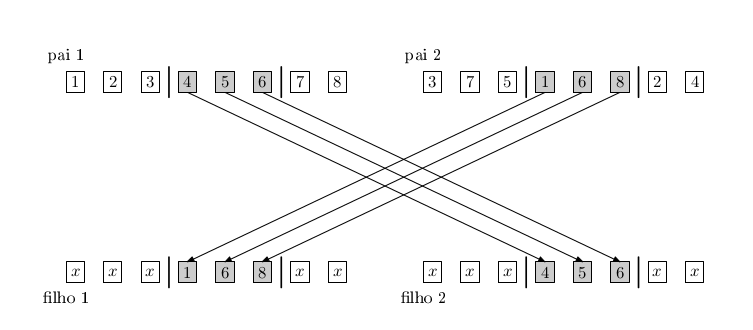
\includegraphics[width = 14cm,keepaspectratio]{img/pmx.png}
		        \caption*{Fonte:\cite{0012-pdf}.}
		        \label{pmx}
	   		\end{figure}

	   		Caso o cromossomo já possua o mesmo número, é escolhido outro número com o mesmo índice do pai que não esteja no cromossomo:
	   		\begin{figure}[h]
				\centering
                \caption{PMX - preenchimento}
		        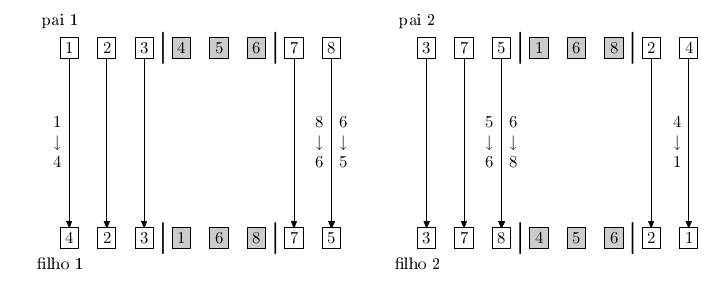
\includegraphics[width = 14cm,keepaspectratio]{img/pmx2.png}		        
		        \caption*{Fonte:\cite{0012-pdf}.}
		        \label{pmx2}
	   		\end{figure}

	   		Por exemplo, como o ``filho 1'' já possui o valor 1, então é pesquisada qual a posição que o valor 1 está neste vetor, no caso da \textbf{figura~\ref{pmx2}} o valor 1 está na posição 4, então o valor na posição 4 do vetor do ``pai 1'' é copiado para a posição 1 do vetor ``filho 1''. No outro exemplo na mesma figura, na terceira posição do vetor do ``filho 2'',  o número 5 já existe na posição 5, sendo assim, o valor que está na posição 5 no vetor ``pai 2'' é o valor 6, mas este valor também existe do vetor ``filho 2'', portanto é pesquisada a posição do valor 6 no vetor ``filho 2'', que neste caso é a posição 6, então copia-se o valor 8 que está na posição 6 do vetor ``pai 2'' para a terceira posição do vetor ``filho 2''. 
	   		Este processo descrito acima é repetido para todos os outros elementos vazios\footnote{Os valores vazios são representados pelos caracteres ``x'' na \textbf{figura~\ref{pmx}}.} dos filhos.
	   		  
		\subsection{Operador de mutação}
			\label{Sem}
			O operador de mutação define como será realizada a mutação de um cromossomo, impedindo que o programa sempre gere os mesmos indivíduos (cromossomos) \cite{0012-pdf}.

			Foi implementado no algoritmo proposto o operador de mutação por troca \textit{exchange mutation} (EM). Ele seleciona dois genes, aleatoriamente, do cromossomo e os troca de posição.

		\subsection{Algoritmo Genético Híbrido}

			Os Algoritmos Genéticos possuem o objetivo de serem robustos, ou seja, são eficientes nas soluções de problemas com complexidade \textit{NP-HARD}, mas, estes algoritmos têm dificuldade em encontrar o caminho ótimo. Para solucionar esse problema foram criados os Algoritmos Genéticos Híbridos.

			Os Algoritmos Genéticos Híbridos consistem em utilizar um outro algoritmo em conjunto com o Algoritmo Genético, produzindo algoritmos eficientes na prática \cite{TravelingTheory}.

        \subsection{Algoritmo \textit{Nearest-Neighbor} (NN)}

            O Algoritmo \textit{Nearest-Neighbor} (NN) é classificado como um algoritmo guloso\footnote{Um algoritmo guloso preza pela menor rota localmente, sem se preocupar com o desempenho da rota globalmente.}.

            O NN é um algoritmo simples de implementação, sua única tarefa é selecionar um vértice e verificar qual vértice ao seu redor está mais próximo, e colocá-lo como próximo vértice a ser visitado. Após isso, esse passo é repetido para o vértice escolhido. 

            O algoritmo NN possui uma complexidade $O(\frac{n^2-n}{2})$, pois faz a comparação com todos os vértices ainda não visitados \cite{NN}.

            Este algoritmo é utilizado na geração da população inicial, sendo que a quantidade de indivíduos gerados por este algoritmo é definido por um parâmetro chamado \textbf{AmountPopulationWithNN}. O valor deste parâmetro deve ser menor ou igual ao valor do parâmetro \textbf{InitialPopulation}, caso o valor seja menor, o restante dos indivíduos da população inicial será gerado de forma aleatória, se o valor for igual, toda a população inicial será gerada pelo algoritmo \textit{Nearest-Neighbor}.  
			
		\chapter{Estado da Arte}
		
			Existem diversos trabalhos sobre a utilização de Algoritmos Genéticos na resolução do problema do TSP. A solução apresentada por \citeonline{0006-pdf} propõe resolver os problemas de roteirização de 
			veículos com entregas fracionadas, problema clássico de roteirização de veículos e com 
			frota heterogênea criando o algoritmo de roteirização de veículos com frota heterogênea, 
			restrições de janelas de tempo e entregas fracionadas (\textit{Heterogeneous Fleet Vehicle 
			Routing Problem with Time Windows and Split Deliveries} - HFVRPTWSD) utilizando Algoritmo 
			Genético (AG).

			Na proposta  apresentada por \citeonline{0011-pdf} para a resolução do \textit{mTSP} com um depósito, foi criado um único cromossomo utilizando o método \textit{two-part}, que será explicado no próximo capítulo. Este método mostrou-se muito eficiente.

			\citeonline{0005-pdf}  mostra que é possível calcular as rotas de múltiplos veículos utilizando AG para igualar o tempo 
			de espera de encomendas de clientes, sendo que a variável ``menor tempo da rota'' não é levada em consideração.

		
		\chapter{Desenvolvimento}
		
		O Algoritmo Genético Híbrido (GANN - \textit{Genetic Algorithm with Nearest Neighbor}) proposto utiliza os conceitos do Algoritmo Genético tradicional em conjunto com o algoritmo  \textit{Nearest-Neighbor} (NN).

		O desenvolvimento do Algoritmo Híbrido foi necessário pois, como ilustra a \textbf{figura~\ref{graf-agestag}},  a população do Algoritmo Genético está convergindo para um indivíduo que não é eficiente o suficiente, comparando com os resultados da base de teste TSPLIB.  

		\begin{figure}[h]
			\centering
            \caption{Evolução da rota utilizando AG com 2000 pontos.}
			\begin{tikzpicture}
			    \begin{axis}[
			    xlabel = Geração,
    			ylabel = {Distância},
			    width=0.8\textwidth,
			    height=10cm,
			    ymajorgrids,
			    x tick label style={/pgf/number format/1000 sep=},
			    scaled y ticks = false,
			    y tick label style={/pgf/number format/fixed,
		      	/pgf/number format/1000 sep = \thinspace % Optional if you want to replace comma as the 1000 separator 
		      	},
		      	legend style={
					legend columns=1,
					    at={(yticklabel cs:-0.1)},
					    anchor=north
					},
			    ]
			    \addplot table[x=Geração,y=Tamanho] {AG.csv};\addlegendentry{AG sem NN}
			    \end{axis}
			\end{tikzpicture}
            \caption*{\textbf{Fonte:} Do autor.}
			\label{graf-agestag}
		\end{figure}

		Portanto, com a utilização do algoritmo \textit{Nearest-Neighbor}, pode-se criar uma boa população inicial, contudo, após a criação desses indivíduos, o Algoritmo Híbrido (Algoritmo Genérico com o  \textit{Nearest-Neighbor}) não consegue evoluir a população, como a \textbf{figura~\ref{figagnn}} ilustra.  

		\begin{figure}[h]
			\centering
            \caption{Evolução da rota com o algoritmo híbrido (GANN).}
			\begin{tikzpicture}
			    \begin{axis}[
			    xlabel = Geração,
    			ylabel = {Distância},
			    width=0.8\textwidth,
			    height=5cm,
			    ymajorgrids,
			    x tick label style={/pgf/number format/1000 sep=},
			    scaled y ticks = false,
			    y tick label style={/pgf/number format/fixed,
		      	/pgf/number format/1000 sep = \thinspace % Optional if you want to replace comma as the 1000 separator 
		      	},
		      	legend style={
					legend columns=1,
					    at={(xticklabel cs:0.5)},
					    anchor=north
					},
			    ]
			    \addplot table[x=Geração,y=Tamanho] {t5.csv};\addlegendentry{AG com NN}
			    \end{axis}
			\end{tikzpicture}
			\caption*{\textbf{Fonte:} Do autor.}
			\label{figagnn}
		\end{figure}


		O algoritmo \textit{Nearest-Neighbor} é utilizado para gerar a quantidade de indivíduos na população inicial definida pelo parâmetro \textit{AmountPopulationWithNN}. Para calcular o número de indivíduos que serão geradas aleatoriamente é utilizado este cálculo:

			\begin{equation}
				\label{cal_ind}
		 		NumeroDeIndividuosAleatorios = InitialPopulation - AmountPopulationWithNN 
		 	\end{equation} 
		
		Sendo que a variável $InitialPopulation$ na \textbf{equação~\ref{cal_ind}} é um parâmetro do algoritmo que armazena a quantidade total de indivíduos que a população inicial deve conter antes do processo de evolução ocorrer, como o cruzamento e a mutação.

        \section{Parâmetros}
        
        Segundo \citeonline{0001-pdf}, os parâmetros são importantes para analisar o comportamento do algoritmo e ajustá-lo para suprir as necessidades do problema. 
        
        No algoritmo GANN foram implementados os seguintes parâmetros:
         
            \begin{itemize}
                \item \textbf{MaxPopulation:} Define o número máximo da população; 
                \item \textbf{InitialPopulation:} Define a quantidade inicial de indivíduos dentro da população, as rotas destes indivíduos serão gerados aleatoriamente. Caso o parâmetro \textit{InitialPopulationWithNN} for \textit{true}, 
                \item \textbf{InitialPopulationWithNN:} Se for igual a \textit{true}, um indivíduo da população inicial será gerado utilizando o algoritmo NN;
                \item \textbf{AmountPopulationWithNN:} Define o número de indivíduos que serão gerados na população inicial utilizando o algoritmo NN;
                \item \textbf{MutationRouteItself:} Se for igual a \textit{true}, a mutação ocorrerá dentro da rota de um caixeiro viajante, ou seja, os pontos da rota de um caixeiro não poderão ser trocados com outros caixeiros. Se for igual a \textit{false}, os pontos poderão ser trocados entre os caixeiros;
                \item \textbf{NNsizePart:} Define o tamanho da área em que os pontos serão gerados, por exemplo, se está variável possuir o valor 100, então será criado um espaço 100x100;
                \item \textbf{NNnPart:} Define o número de áreas em que o espaço será dividido para a utilização do algoritmo NN;
                \item \textbf{AmountMutation:} Define quantos pares de vértices serão trocados por uma mutação.
                \item \textbf{RateMutation:} Define a probabilidade de um indivíduo da população sofrer mutação;
                \item \textbf{RateGeneration:} Define a chance de adicionar ou substituir novos indivíduos na população, por exemplo, se o parâmetro \textit{MaxPopulation} for maior que o valor do parâmetro \textit{Initial Population}, então os dois novos indivíduos que serão gerados por meio do cruzamento terão chances de substituir um indivíduo da população, mesmo que o número máximo da população não tenha sido atingido, ou serão adicionados sem substituir nenhum indivíduo. Após a população atingir o número máximo permitido pelo parâmetro \textit{MaxPopulation}, apenas ocorrerá substituição dos piores indivíduos;
                \item \textbf{RateSalesmanMutation:} Define a probabilidade de mutação no número de pontos que cada caixeiro irá visitar, ou seja, irá afetar a segunda parte do cromossomo (\textit{two-part});
                \item \textbf{Generation:} Define o número de iterações que o programa realizará;
                \item \textbf{Deposit:} Define qual ponto será o depósito no qual os caixeiros irão sair;
                \item \textbf{Salesman:} Define o número de caixeiros viajantes;
                \item \textbf{SaveBetterChromo:} Se for igual a \textit{true}, o melhor indivíduo não poderá sofrer mutação;
                \item \textbf{AmountThread:} Define o número de \textit{threads} para processar as áreas do NN.
            \end{itemize}   

		\section {\textit{Nearest-Neighbor} modificado}
            \label{NNMod}
		O algoritmo \textit{Nearest-Neighbor} (NN) possui uma alta complexidade. Para resolver este problema, o plano cartesiano pode ser dividido em inúmeras áreas de tamanhos iguais, sendo que o número de áreas é definido pelo parâmetro \textit{NNnPart}, sendo sempre $NNnPart > 0$. 
		Com isso, pode-se aplicar o NN em cada área, sendo assim, os pontos de uma área não podem ser comparados com os pontos de outras áreas reduzindo assim a complexidade para, na melhor hipótese, aproximadamente, $O(\frac{n^2-kn}{2k^2}k)$, sendo $n$ o número total de pontos e $k$ o número de áreas, e na pior hipótese $O(\frac{n^2-n}{2})$, quando todos os pontos estão em apenas uma área. 
		
		O tamanho do plano cartesiano é definido pelo parâmetro $NNsizePart$, utilizando o NN, o plano cartesiano será dividido em linhas e colunas, sendo que cada área será de tamanho igual, por exemplo, se o parâmetro $NNnPart = 4$, então o plano cartesiano com os vértices será dividido em 4 linhas e 4 colunas.  
		
		
		\section{Estrutura do cromossomo (indivíduo) - \textit{two-part}}
		

			Cada cromossomo representa uma possível solução para o problema, então, para definir a estrutura do cromossomo do algoritmo foi utilizado o método \textit{two-part}.

			O \textit{two-part} consiste em dividir o cromossomo em duas partes, uma parte armazena as informações da rota e a outra a informação dos caixeiros. Considere o cromossomo da \textbf{figura~\ref{imgtwopart}}.
			
            \begin{center}
                \begin{figure}[h]

                \caption{Cromossomo representado pelo método \textit{two-part}.}
				\centering
                \begin{tikzpicture}
					\tikzstyle{every path}=[very thick]

					\edef\sizetape{0.65cm}
					\tikzstyle{tmtape}=[draw,minimum size=\sizetape]
					\tikzstyle{tmhead}=[blue,draw,minimum size=\sizetape]
					\tikzstyle{l} = [draw, -latex',thick]
					%% Draw TM tape
					\begin{scope}[start chain=1 going right,node distance=-0.15mm]
					    \node [on chain=1,tmtape] (1){1};
					    \node [on chain=1,tmtape] (2){9};
					    \node [on chain=1,tmtape] {10};
					    \node [on chain=1,tmtape] {3};
					    \node [on chain=1,tmtape] {11};
					    \node [on chain=1,tmtape] {5};
					    \node [on chain=1,tmtape] {4};
					    \node [on chain=1,tmtape] {2};
					    \node [on chain=1,tmtape] {6};
					    \node [on chain=1,tmtape] {7};
					    \node [on chain=1,tmtape] {8};
					    \node [on chain=1,tmhead] (01){2};
					    \node [on chain=1,tmhead] {6};
					    \node [on chain=1,tmhead] {3};
					\end{scope}

				\end{tikzpicture}
				\caption*{\textbf{Fonte:} Do autor.}
                \label{imgtwopart}
			\end{figure}
            \end{center}

			Os três últimos genes representam os caixeiros. Neste exemplo foi definido o ponto de partida como sendo o 0. Seguindo este raciocínio, o primeiro caixeiro terá que sair do ponto 0 e visitar dois pontos, ou seja, os pontos 1 e 9 e retornar ao ponto 0, já o segundo caixeiro terá que sair do ponto 0 e visitar seis pontos, os pontos 10, 3, 11, 5, 4 e 2 e retornar ao ponto 0 e o último caixeiro terá que sair do ponto 0 e visitar três pontos, os pontos 6,7 e 8 e retornar ao ponto 0 (\textbf{figura~\ref{two-part}}).
			\\
			\begin{center}
			\begin{figure}[h]
			\centering
            \caption{Cromossomo - \textit{two-part}.} 
			\begin{tikzpicture}
				\tikzstyle{every path}=[very thick]

				\edef\sizetape{0.65cm}
				\tikzstyle{tmtape}=[draw,minimum size=\sizetape]
				\tikzstyle{tmheadgreen}=[green,draw,minimum size=\sizetape]
				\tikzstyle{tmheadblue}=[blue,draw,minimum size=\sizetape]
				\tikzstyle{tmheadred}=[red,draw,minimum size=\sizetape]
				\tikzstyle{l} = [green,draw, -latex',thick]
				\tikzstyle{la} = [red,draw, -latex',thick]
				\tikzstyle{lb} = [blue, draw, -latex',thick]
				%% Draw TM tape
				\begin{scope}[start chain=1 going right,node distance=-0.15mm]
				    \node [on chain=1,tmtape] (1){1};
				    \node [on chain=1,tmtape] (2){9};
				    \node [on chain=1,tmtape] (3){10};
				    \node [on chain=1,tmtape] (4){3};
				    \node [on chain=1,tmtape] (5){11};
				    \node [on chain=1,tmtape] (6){5};
				    \node [on chain=1,tmtape] (7){4};
				    \node [on chain=1,tmtape] (8){2};
				    \node [on chain=1,tmtape] (9){6};
				    \node [on chain=1,tmtape] (10){7};
				    \node [on chain=1,tmtape] (11){8};
				    \node [on chain=1,tmheadgreen] (01){2};
				    \node [on chain=1,tmheadred] (02){6};
				    \node [on chain=1,tmheadblue] (03){3};
				   
				    \draw [l] (01.south) -- ++(0,-0.5) -| (1.south);
				    \draw [l] (01.south) -- ++(0,-0.5) -| (2.south);
				
					\draw [la] (02.south) -- ++(0,-1) -| (3.south);
				    \draw [la] (02.south) -- ++(0,-1) -| (4.south);
				    \draw [la] (02.south) -- ++(0,-1) -| (5.south);
				    \draw [la] (02.south) -- ++(0,-1) -| (6.south);
				    \draw [la] (02.south) -- ++(0,-1) -| (7.south);
				    \draw [la] (02.south) -- ++(0,-1) -| (8.south);

				    \draw [lb] (03.south) -- ++(0,-1.5) -| (9.south);
				    \draw [lb] (03.south) -- ++(0,-1.5) -| (10.south);
				    \draw [lb] (03.south) -- ++(0,-1.5) -| (11.south);
				\end{scope}
			\end{tikzpicture}
				\caption*{\textbf{Fonte:} Do autor.}
				\label{two-part}
			\end{figure}
			
			\end{center}

            No algoritmo híbrido desenvolvido neste trabalho, o número de pontos serão distribuídos entre os caixeiros de forma igual caso o indivíduo seja gerado aleatoriamente, se o indivíduo foi gerado pelo algoritmo \textit{Nearest Neighbor} modificado, as áreas que este algoritmo gerou, explicado na seção \ref{NNMod}, serão distribuídas de forma igual, permitindo que cada caixeiro fique responsável por visitar uma mesma quantidade de áreas que os outros.
		       
	   	
	   	\section{Avaliação do Indivíduo (\textit{fitness})}

		Para cada novo indivíduo gerado, é calculada a distância dos pontos da rota, por meio da distância euclidiana bidimensional que pode ser definida pela \textbf{equação ~\ref{eq-eclidiana}}.

		\begin{equation}
			d = \sqrt{(x_2-x_1)^2 + (y_2-y_1)^2}
			\label{eq-eclidiana}
		\end{equation}

		Sendo que a variável $d$ é a distância entre dois vértices do grafo, o valor $d$ se torna o valor do peso da aresta que liga os dois vértices.

		O cálculo da distância total ($dt$) é dado por:

		\begin{equation}
			d = \sum_{j=1}^{c} \sum_{i=1}^{a_j-1} \sqrt{(vcx_{ji}-vcx_{ji+1})^2 + (vcy_{ji}-vcy_{ji+1})^2}
			\label{eq-ecli1}
		\end{equation}
		\begin{equation}
			dt = d + \sum_{i=1}^{c} (\sqrt{(depX-vcx_{i1})^2 + (depY-vcy_{i1})^2} + \sqrt{(depX-vcx_{iq})^2 + (depY-vcy_{iq})^2})
			\label{eq-ecli2}
		\end{equation}

		Considerando que $a$ é um vetor que representa o número total de vértices de cada caixeiro, sem considerar as  arestas que estão vinculadas ao depósito, $vcx$ e $vcy$ são matrizes de duas dimensões, sendo que o primeiro índice representa o caixeiro e o segundo índice representa o vértice pertencente ao caixeiro do primeiro índice, que armazenam os valores de $x$ e $y$ respectivamente. As variáveis $depX$ e $depY$ armazenam as posições do depósito, onde os caixeiros irão iniciar seus trajetos, assim:
		\begin{equation}
			vcx, vcy, depX, depY \in \mathbb{R}   
			\label{eq-ecli4}
		\end{equation}

		A variável $c$ representa o número de caixeiros viajantes, e a variável $q$ representa o valor do último vértice do caixeiro.

		Na \textbf{equação~\ref{eq-ecli1}} é calculada a distância das conexões entre os vértices, não considerando o depósito. Já na \textbf{equação~\ref{eq-ecli2}} é adicionada a distância do depósito para o primeiro e o último vértice da rota de cada caixeiro, finalizando o cálculo da distância total.

		O algoritmo considera o melhor indivíduo aquele que tiver a menor distância total. 

		\section{Cruzamento}

			O programa proposto utiliza o operador de cruzamento PMX, descrito no capítulo (\ref{Spmx}). 
			
			A cada iteração (geração) é realizado um cruzamento, para isso são selecionados, aleatoriamente, dois cromossomos da população. No cruzamento são gerados dois novos indivíduos, esses indivíduos serão avalizados pela função \textit{fitness} e inseridos na população.

		\section{Mutação}

			O programa proposto utiliza o operador de mutação EM (\textit{Exchange Mutation}), descrito no capítulo~\ref{Sem}. A chance do cromossomo sofrer mutação é definida no parâmetro $RateMutation$, sendo que $\{RateMutation \in \mathbb{R}~|~ 0 \leq RateMutation \leq 1\}$. O parâmetro  $AmountMutation$, considerando que  $\{AmountMutation \in \mathbb{N}^*\}$, estabelece quantos pares de genes (vértices) do cromossomo serão trocados.
						
		
			
		\section{Desempenho}
		
		Para mensurar o desempenho do algoritmo foram realizados diversos testes com parâmetros diferentes, levando em consideração o tamanho da rota e o tempo de execução. A base de testes TSPLIB foi utilizada apenas para validar o algoritmo, pois esta base apenas contém testes para o problema do caixeiro viajante, sendo que o algoritmo proposto tenta solucionar o problema dos múltiplos caixeiros viajantes. 
		
        \subsection{Requisitos de Sistema}

		O algoritmo foi implementado utilizando a linguagem C++ e compilado com o compilador GCC versão 4.8, utilizando os parâmetros \textit{-pthread -O3 -std=c++11}. Os resultados gráficos das rotas foram gerados pela biblioteca BITMAPIMG\footnote{A biblioteca BITMAPIMG foi desenvolvida pelo autor e está disponível em \url{https://github.com/VictorCarlquist/BITMAPIMG}.}. Foi desenvolvida esta biblioteca, pois o \textit{software} \textit{gnuplot} utilizado inicialmente para gerar as figuras não tinha um bom desempenho para plotar mais de 100.000 pontos, e os testes estavam consumindo muito tempo para plotar a imagem dos resultados e, também,  não foi encontrada uma biblioteca para plotar as figuras de uma maneira simples. Portanto, foi desenvolvida a biblioteca BITMAPIMG com o objetivo de plotar linhas e pontos de maneira simples, com isso foi possível gerar as figuras mais rapidamente.

		O computador que executou os testes possui processador Intel\textregistered Core\texttrademark ~i5 2,4GHz, 4GB de memória RAM. É necessário ressaltar que os tempos de execuções entre os resultados da base de testes TSPLIB e o algoritmo desenvolvido pelo autor possuem discrepâncias, pois as arquiteturas dos processadores são diferentes, exceto no teste PR2392, portanto, os testes entre esses resultados são utilizados para, apenas, validar o algoritmo.

		\subsection{Resultados do Problema do Caixeiro Viajante (TSP)}

		É necessário medir o desempenho do Algoritmo Híbrido contra o Problema do Caixeiro Viajante, pois com os resultados é possível se ter uma base de comparação para constatar se o Algoritmo Híbrido está sendo executado corretamente, já que não foi possível encontrar nenhuma base de testes para o problema dos múltiplos caixeiros viajantes.

        \begin{figure}[h]
            \centering
            \caption{TSPLIB - Imagem gerada pelo algoritmo LKH, Argentina.}
            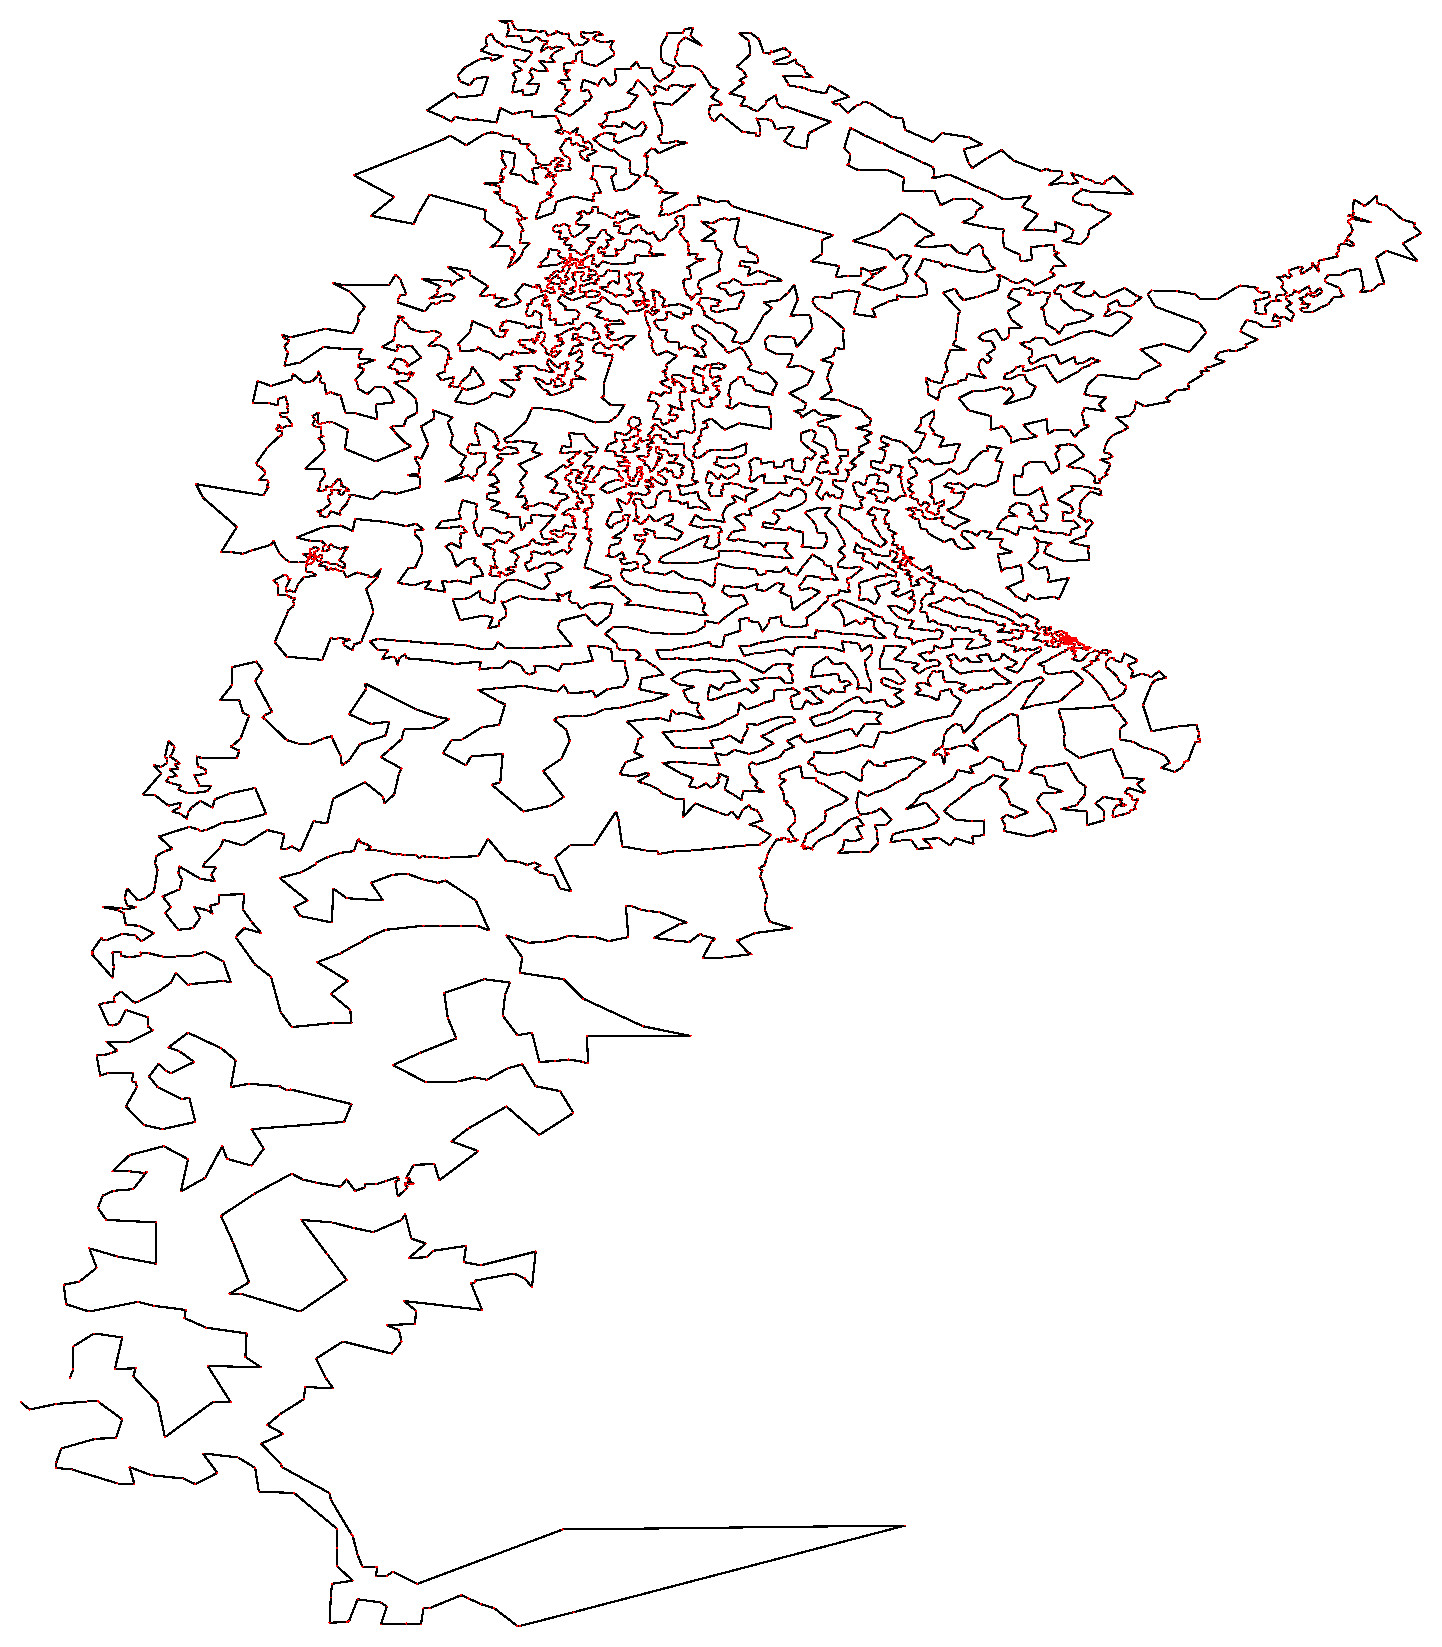
\includegraphics[width = 8cm,keepaspectratio]{img/artour.jpg}
            \caption*{\textbf{Fonte:} TSPLIB.}
            \label{figargentina}
        \end{figure}

		Foram utilizados três testes da base de dados do \textit{TSPLIB}. Os testes escolhidos contém todas as cidades da Argentina (9152 cidades), China (71.009 cidades) e um teste denominado PR2392 (2392 pontos) fornecido pela \textit{Tektronics Incorporated} e armazenado no \textit{TSPLIB}. 
        
        A rota ótima para o Problema do Caixeiro Viajante (TSP) utilizando a Argentina é de 837.479 km (\textbf{figura~\ref{figargentina}}). O melhor algoritmo para este problema encontrou a rota ótima em 24.301 segundos (aproximadamente 6 horas e 45 minutos) sendo executado em uma arquitetura Sun Ultra 80 450 MHz.
        \newpage
        \begin{figure}[h]
            \centering
            \caption{Teste utilizando o Algoritmo Genético - Argentina.}
            \includegraphics[width = 8cm,keepaspectratio]{a1.jpg}
            \caption*{\textbf{Fonte:} Do autor.}
            \label{figa1}
        \end{figure}

        \begin{figure}[h]
            \centering
            \caption{Teste utilizando o Algoritmo \textit{Nearest-Neighbor} - Argentina.}
            \includegraphics[width = 8cm,keepaspectratio]{ANN0.jpg}
            \caption*{\textbf{Fonte:} Do autor.}
            \label{figANN0}
        \end{figure}		

		Executando o teste com as cidades da Argentina utilizando o Algoritmo Genético ``tradicional'', foi gerada uma rota com tamanho de 67.889.725,27 km (\textbf{figura~\ref{figa1}}) e, com o Algoritmo Híbrido (GANN), gerou uma rota com tamanho de 1.182.405,53 km (\textbf{figura~\ref{figANN0}}), ambos com apenas um caixeiro. Isso demonstra que o algoritmo desenvolvido pode ser utilizado para se ter uma solução rápida, mas com uma qualidade menor; no Problema do Caixeiro Viajante, a rota gerada foi 41,18\% maior, tendo um tempo de execução de 13,41 segundos. Utilizando apenas o \textit{Nearest-Neighbor} modificado, o tempo de execução é reduzido para, aproximadamente, 1,16 segundo com o mesmo tamanho de 1.182.405,53 km.

   		\begin{figure}[h]
			\centering
            \caption{Teste utilizando o Algoritmo Genético - China.}
	        \includegraphics[width = 7cm,keepaspectratio]{t1.jpg}
	        \caption*{\textbf{Fonte:} Do autor.}
	        \label{figt1}
   		\end{figure}

        Os teste com as cidades da China utilizando apenas o Algoritmo Genético resultaram em uma rota de 804.136.489,44 km (\textbf{figura~\ref{figt1}}), executado em 97,53 segundos com 8000 gerações, e utilizando o GANN, o tamanho da rota foi de 5.884.954,34 km, executado em 75,93 segundos (\textbf{figura~\ref{figtNN0}}). Uma rota ótima já encontrada, segundo o TSPLIB, é de 4.566.563 km com o tempo de execução de 72.945 segundos utilizando um processador Sun Ultra 80 450 MHz.
        \begin{figure}[h]
            \centering
            \caption{Teste utilizando o GANN - China.}
            \includegraphics[width = 8cm,keepaspectratio]{tNN0.jpg}
            \legend{Fonte: o autor.}
            \label{figtNN0}
        \end{figure}

        
   		\subsubsection{GANN \textit{versus} LKH}

		O melhor algoritmo que é utilizado para gerar as menores rotas do TSPLIB é o LKH (Lin-Kernighan). Este algoritmo é especializado em \textit{exchanges} (trocas), ou seja, são realizadas diversas trocas de arestas entre os vértices, obtendo uma rota mais eficiente, demonstrando ser um bom algoritmo para resolver o Problema do Caixeiro Viajante \cite{LKH}. 

		\begin{figure}[h]
			\centering
            \caption{Resultado do teste PR2392 gerado por GANN.}
		    \includegraphics[width = 8cm,keepaspectratio]{pr.jpg}
		    \caption*{\textbf{Fonte:} Do autor.}
		    \label{figpa}
		\end{figure}

		Foi executado o teste PR2392 (2392 pontos) utilizando o LKH e o GANN, sendo que ambos foram executados no mesmo computador\footnote{Processador Intel\textregistered Core\texttrademark ~i5 2,4 Hz com 4GB de memória RAM.}. Neste teste o LKH gerou uma rota com 378.032 km em 0,70 segundos, já o algoritmo GANN gerou 481.994,76 km em 0,30 segundos (\textbf{figura~\ref{figpa}}).
		O algoritmo GANN, apesar de não gerar a melhor rota, é eficiente em encontrar uma solução aceitável em um menor tempo.

        \newpage
		\subsection{Resultados do Problema dos Múltiplos Caixeiros Viajantes (mTSP)}	

        Nas próximas seções serão demonstrados os resultados que o algoritmo híbrido desenvolvido obteve em gerar uma solução para o Problema dos Múltiplos Caixeiros Viajantes.

		\subsubsection{Múltiplos Caixeiros - GANN}
		
		O Algoritmo Híbrido mostrou-se eficiente na solução do Problema dos Múltiplos Caixeiros Viajantes (mTSP), pois o tempo de execução se manteve o mesmo com diversos caixeiros, em média 175 segundos.

		\begin{figure}[h]
			\centering
            \caption{Evolução da rota com diversos caixeiros viajantes (GANN).}
			\begin{tikzpicture}
			    \begin{axis}[
			    xlabel = Geração,
    			ylabel = {Distância},
			    width=0.77\textwidth,
			    height=5cm,
			    ymajorgrids,
			    x tick label style={/pgf/number format/1000 sep=},
			    scaled y ticks = false,
			    y tick label style={/pgf/number format/fixed,
		      	/pgf/number format/1000 sep = \thinspace % Optional if you want to replace comma as the 1000 separator 
		      	},
		      	legend style={
					legend columns=1,
					    at={(yticklabel cs:-0.1)},
					    anchor=north
					},
			    ]
			    %\addplot table[x=Geração,y=Tamanho] {t1a.csv};\addlegendentry{AG com NN}
			    \addplot table[x=Geração,y=Tamanho] {via1.csv};\addlegendentry{GANN com 2 viajantes}
			    \addplot table[x=Geração,y=Tamanho] {via2.csv};\addlegendentry{GANN com 4 viajantes}
			    \addplot table[x=Geração,y=Tamanho] {via3.csv};\addlegendentry{GANN com 8 viajantes}
			    
			    \end{axis}
			\end{tikzpicture}
			\caption*{\textbf{Fonte:} Do autor.}
			\label{figmult}
		\end{figure}

        Como a \textbf{figura~\ref{figmult}} apresenta, o tamanho da rota aumenta conforme o número de caixeiros também aumenta, porque é necessário adicionar um caminho de saída do depósito e um outro caminho de entrada para cada caixeiro, portanto, quanto maior for o número de caixeiros, mais caminhos de entrada e saída serão adicionados, influenciando no tamanho da rota.

        \newpage
		\subsubsection{Múltiplos Caixeiros - GA}

		Foram realizados alguns testes para verificar o comportamento do Algoritmo Genético em resolver o Problema dos Múltiplos Caixeiros Viajantes.

		\begin{figure}[h]
			\centering
            \caption{Evolução da rota com diversos viajantes (GA).}
			\begin{tikzpicture}
			    \begin{axis}[
			    xlabel = Geração,
    			ylabel = {Distância},
			    width=0.77\textwidth,
			    height=10cm,
			    ymajorgrids,
			    x tick label style={/pgf/number format/1000 sep=},
			    scaled y ticks = false,
			    y tick label style={/pgf/number format/fixed,
		      	/pgf/number format/1000 sep = \thinspace % Optional if you want to replace comma as the 1000 separator 
		      	},
		      	legend style={
					legend columns=1,
					    at={(yticklabel cs:-0.1)},
					    anchor=north
					},
			    ]
			    %\addplot table[x=Geração,y=Tamanho] {t1a.csv};\addlegendentry{AG com NN}
			    \addplot table[x=Geração,y=Tamanho] {t2.csv};\addlegendentry{AG com 2 viajantes}
			    \addplot table[x=Geração,y=Tamanho] {t3.csv};\addlegendentry{AG com 4 viajantes}
			    \addplot table[x=Geração,y=Tamanho] {t4.csv};\addlegendentry{AG com 8 viajantes}
			    \end{axis}
			\end{tikzpicture}
			\caption*{\textbf{Fonte:} Do autor.}
			\label{figgaga}
		\end{figure}

		A \textbf{figura~\ref{figgaga}} ilustra que, apesar de que cada teste possui um número de caixeiros diferentes, todos os resultados tem um comportamento semelhante. Vale salientar que o resultado com 8 caixeiros iniciou-se com a maior rota e terminou com o melhor resultado das 3 soluções expostas nesta figura.

		\subsection{Threads}

		Uma \textit{thread} possui um ID, um contador de programa, um conjunto de registradores e uma pilha. Também compartilha com outras \textit{threads} em um mesmo processo a seção de código, seção de dados e outros recursos do sistema operacional (SO), como arquivos abertos e sinais. 
		O processo tendo mais de uma \textit{thread} significa que é possível realizar mais de uma tarefa ao mesmo tempo \cite{THREAD}.

			\subsubsection{\textit{Threads} (GANN)}

			Foram implementados \textit{threads} para otimizar o tempo de execução do \textit{Nearest-Neighbor}. 

			O parâmetro \textit{NNnPart} define a quantidade de áreas em que o espaço será dividido, essas áreas serão distribuídas igualmente para cada \textit{thread}, dividindo a carga de processamento entre os núcleos, caso o \textit{hardware} tenha mais que um processador ou núcleo (\textit{core}).

			\begin{figure}[h!]
				\centering
                \caption{Desempenho do algoritmo utilizando \textit{threads}.}
				\begin{tikzpicture}
				    \begin{axis}[
				    xlabel = {\textup{N}\ensuremath{^\circ} de \textit{threads}},
	    			ylabel = {Tempo ($s$)},
				    width=0.77\textwidth,
				    height=5cm,
				    ymajorgrids,
				    x tick label style={/pgf/number format/1000 sep=},
				    scaled y ticks = false,
				    y tick label style={/pgf/number format/fixed,
			      	/pgf/number format/1000 sep = \thinspace % Optional if you want to replace comma as the 1000 separator 
			      	},
			      	ybar interval=0.7,
			      	legend style={
						legend columns=1,
						    at={(yticklabel cs:-0.1)},
						    anchor=north
						},
				    ]
				    \addplot table[x=thread,y=tempo] {a9.csv};\addlegendentry{GANN - Teste}
				    \end{axis}
				\end{tikzpicture}
				\caption*{\textbf{Fonte:} Do autor.}
				\label{figthread}
			\end{figure}

            O algoritmo \textit{Nearest Neighbor} divide o plano cartesiano em diversas áreas, assim, cada área pode ser processada por uma \textit{thread}, podendo aumentar o desempenho do algoritmo na geração da população inicial. Como a \textbf{figura~\ref{figthread}} demonstra, nos 4 testes realizados, a utilização das \textit{threads} não teve impacto no tempo de execução, pois a implementação do algoritmo está tendo um falso paralelismo que pode estar sendo causado pelo acesso à memória RAM (\textit{Random Access Memory}) pelas múltiplas \textit{threads}, mas a razão deste resultado precisará ser investigada em um trabalho futuro, pois não é um problema trivial.  


	\chapter{Conclusão e trabalhos futuros}
		
	O Algoritmo Híbrido desenvolvido apresentou um bom tempo de execução para gerar uma solução para o problema dos múltiplos caixeiros. Pode-se notar nas imagens das rotas que ainda é possível gerar rotas menores, mostrando que o algoritmo ainda pode ser otimizado.

    Como apresentado nesta pesquisa, o Algoritmo Genético mostrou-se eficiente em uma população gerada aleatoriamente, mas com a utilização do algoritmo \textit{Nearest Neighbor} modificado, para gerar a população inicial, o Algoritmo Genético não consegue evoluir a população com eficácia, pois são necessárias muitas gerações para haver uma melhoria na rota.

    De fato, com este algoritmo é possível obter uma noção do tamanho da rota, podendo ser utilizado para comparar grafos diferentes e auxiliar na escolha do grafo que possui a menor rota.

    Apesar de não ser o objetivo do algoritmo resolver o problema de um caixeiro viajante, ele também se mostrou eficiente em encontrar uma rota com tempo de execução pequeno.

    Portanto, este trabalho demonstra que um algoritmo híbrido pode ser utilizado para solucionar o Problema dos Múltiplos Caixeiros Viajantes.  

    Como trabalho futuro, poderiam ser adicionadas novas estratégias para gerar a população inicial e realização dos cruzamentos dos cromossomos. Com essas implementações a probabilidade do Algoritmo Genético evoluir a população poderia aumentar.

    Uma segunda abordagem para otimizar a solução poderia ser adicionar novas análises ao algoritmo \textit{Nearest Neighbor}, fazendo com que a análise de seus vizinhos seja melhor gerenciada, podendo eliminar o Algoritmo Genético.

    A implementação de \textit{threads} utilizando GPUs (\textit{Graphics Processing Unit}) poderia deixar mais rápido o algoritmo, já que cada geração do algoritmo genético ou a otimização de cada parte (área) do \textit{Nearest Neighbor} pode ocorrer separadamente.
    
%\begin{comment}
	%\section{Modelagem real}
	%\chapter{Conclusão}
%\end{comment}
	\postextual
	\bibliography{refs}

	\apendices
	\chapter{Código Fonte - main.cpp}
	\lstinputlisting{../code/algo_genetico_comum/agc/agc/main.cpp}
	\chapter{Código Fonte - ga.h}
	\lstinputlisting{../code/algo_genetico_comum/agc/agc/ga.h}
	\chapter{Código Fonte - ga.cpp}
	\lstinputlisting{../code/algo_genetico_comum/agc/agc/ga.cpp}

\end{document}
